\documentclass[oneside,final,14pt]{extreport}

%% my command
%%%%%%%%%%%%%%
% Путь к файлу с изображениями
\newcommand{\picPath}{pictures}
% Величина отступа
\newcommand{\indentSpace}{1.25cm}
% Сокращения
\newcommand{\urlTitle}{ $-$ URL: }
%%%%%%%%%%%%%%%


% Изменяем шрифт
\usepackage{fontspec}
\setmainfont{Times New Roman}
\listfiles

% Полуторный интервал
\linespread{1.6}

% Отступ
\setlength\parindent{\indentSpace}

% Математика
\usepackage{mathtools}


% Картинки
\usepackage{graphicx}
\usepackage{subcaption}

% Языковой пакет
\usepackage[russianb]{babel}

% Таблицы
\usepackage{tabularx}

% Настройка подписей к фигурам
% Меняем заголовки картинок
\usepackage[ labelsep= endash]{caption}
\captionsetup{%
   figurename= Рисунок,
   tablename= Таблица,
   justification= centering, singlelinecheck=false
}         

\captionsetup[table]
{
justification= raggedright, singlelinecheck=false
}
% Кирилица в подфигурах
\renewcommand{\thesubfigure}{\asbuk{subfigure}}
% разделитель в подфигурах - правая скобка
\DeclareCaptionLabelSeparator{r_paranthesis}{)\quad }
\captionsetup[subfigure]{labelformat=simple, labelsep=r_paranthesis}

% Добавляем итератор \asbuk,
% чтобы использовать кирилицу
% как маркеры
\usepackage{enumitem}
\makeatletter
\AddEnumerateCounter{\asbuk}{\russian@alph}{щ}
\makeatother

% Меняем маркеры в перечислениях
% Списки уровня 1
\setlist[enumerate,1]{label=\arabic*),ref=\arabic*}
% Списки уровня 2
\setlist[enumerate,2]{label=\asbuk*),ref=\asbuk*}
% Перечисления
\setlist[itemize,1]{label=$-$}
% Удаляем отступы перед и после
% списка
\setlist[itemize]{noitemsep, topsep=0pt}
\setlist[enumerate]{noitemsep, topsep=0pt}

% Красная строка в начале главы
\usepackage{indentfirst}

% Убиваем перенос
\usepackage[none]{hyphenat}

% Перенос длинных ссылок
\usepackage[hyphens]{url}
\urlstyle{same}

% Выравнивание по ширине
\usepackage{microtype}

%\usepackage[fontfamily=courier]{fancyvrb}
%\usepackage{verbatim}%     configurable verbatim
% \makeatletter
%  \def\verbatim@font{\normalfont\sffamily% select the font
%                     \let\do\do@noligs
%                     \verbatim@nolig@list}
%\makeatother

% Границы
\usepackage{vmargin}
\setpapersize{A4}
% отступы
%\setmarginsrb 
%{3cm} % левый
%{2cm} % верхний
%{1cm} % Правый
%{2cm} % Нижний
%{0pt}{0mm} % Высота - отступ верхнего колонтитула
%{0pt}{0mm} % Высота - отступ нижнего  колонтитула

\setlength\hoffset{0cm}
\setlength\voffset{0cm}
\usepackage[top=2cm, bottom=2cm, left=3cm, right=2cm,
]{geometry}
 		
% Настройка заглавиий
\addto\captionsrussian{% Replace "english" with the language you use
  \renewcommand{\contentsname}% содержания
    {\hfill\bfseries
    СОДЕРЖАНИЕ
	\hfill    
    }%
   \renewcommand{\bibname}% списка источников
    {\hfill\bfseries
    	СПИСОК ИСПОЛЬЗОВАННЫХ ИСТОЧНИКОВ
	\hfill
	}% 
}%\

%\renewcommand{\contentsname}{\hfill\bfseries СОДЕРЖАНИЕ \hfill} 

% Настройка  заглавий в главах
\usepackage{titlesec}


%\titleformat
%{\chapter} % command
%[display]
%{
%\bfseries
%} % format
%{
%\thechapter.
%} 	% label
%{ 
%	0 pt
%} % sep
%{    
%\centering
%} % before-code

\titleformat{\chapter}
			[block]
            {\bfseries }
            {\hspace{\indentSpace}\thechapter}
            {1em}
            {\vspace{0mm} }
            [\vspace{14pt}]% Отступ после
% Начальный сдвиг заголовка 50 pt = 1.763888888cm.
% Второй параметр- сдвиг до = 2cm - 50pt
\titlespacing{\chapter}{0pt}
{-0.2361cm}{0pt}

\titleformat{\section}[block]
{\bfseries}{\hspace{\indentSpace}\thesection}{1em}{}

%\titlespacing{\section}{0pt}{0pt}{0pt}

\titleformat{\subsection}[block]
{\bfseries}{\hspace{\indentSpace}\thesubsection}{1em}{}

%\titlespacing{\subsection}{0pt}{0pt}{0pt}

%\titleformat{\section}
%            {\bfseries}
%            {\thechapter.\hspace{1em}}
%            {0pt}
%            {\centering
%            \vspace{0mm} }
%            [\vspace{14pt}]% Отступ после
%\titlespacing{\section}{0pt}{-50pt}{0pt}

% Конец настройка заглавий

% Форматирование списка источников
% Bibl label
\makeatletter
\renewcommand*{\@biblabel}[1]{\indent#1}
\makeatother

% Убрать отсупы в списке источников
\usepackage{lipsum}

% ADD THE FOLLOWING COUPLE LINES INTO YOUR PREAMBLE
%\let\OLDthebibliography\thebibliography
%\renewcommand\thebibliography[1]{
% \OLDthebibliography{#1}
%  \setlength{\parskip}{0pt}
%  \setlength{\itemsep}{0pt plus 0.3ex}
%}

% Change indent
\usepackage{etoolbox}
\patchcmd{\thebibliography}
  {\advance\leftmargin\labelsep}
  {\leftmargin=0pt\itemindent=\labelwidth\advance\itemindent\labelsep}
  {}{}
  
% Define separations
\patchcmd{\thebibliography}{\sloppy}{\itemsep -0.28cm \parsep 0pt \sloppy}{}{}
  



% Добавить точки в оглавление
\usepackage{tocstyle}
\newcommand{\autodot}{}


% Чтобы картинки вставляись
% куда надо
\usepackage{float}

% Для вычисления кол-ва страниц
\usepackage{lastpage}

% Для вычисления кол-ва рисунков и таблиц
%%%
\usepackage{etoolbox}

\newcounter{totfigures}
\newcounter{tottables}

\providecommand\totfig{} 
\providecommand\tottab{}

\makeatletter
\AtEndDocument{%
  \addtocounter{totfigures}{\value{figure}}%
  \addtocounter{tottables}{\value{table}}%
  \immediate\write\@mainaux{%
    \string\gdef\string\totfig{\number\value{totfigures}}%
    \string\gdef\string\tottab{\number\value{tottables}}%
  }%
}
\makeatother

\pretocmd{\chapter}{\addtocounter{totfigures}{\value{figure}}\setcounter{figure}{0}}{}{}
\pretocmd{\chapter}{\addtocounter{tottables}{\value{table}}\setcounter{table}{0}}{}{}
%%%

% Режим релиза
\sloppy
\usepackage{layout}

%\renewcommand{\arraystretch}{1.6}

\newcommand{\cmmnt}[1]{\ignorespaces}
\newcommand{\bs}{\boldsymbol}
\usepackage{breqn}

% Change intemize intend
\usepackage{calc}


\newlength{\mylength}
\settowidth{\mylength}{$-$\textvisiblespace}

\setlist{itemindent= \mylength + \indentSpace ,leftmargin=0pt}


\begin{document}
\tableofcontents
\newpage
\begin{center}
\bfseries ВВЕДЕНИЕ
\end{center}
\addcontentsline{toc}{chapter}{Введение}
Клонирование голоса – популярная задача, используемая для

\begin{itemize}
    \item помощи людям, потерявщим свой голос;
    \item автоматическое озвучивания фильмов / аудиокниг;
    \item реалистичного перевода с сохранением голоса говорящего.
\end{itemize}

Известный метод решения данной задачи - нейронные сети, решающие сразу несколько подзадач внутри себя: генерация голоса (Text To Speech), идентификация спикера (Speaker Identification) и вокализации MEL-спектрограмм. Объединяя эти три задачи и подготавливая специальный датасет, задача в некотором приближении была решена на английском языке\cite{bib:voice_cloning}. Задача данной работы -  реализация алгоритма клонирования голоса на русском языке в условиях ограниченности обучающего набора данных. Код работы в открытом доступе доступен на github\cite{bib:Danya_voice_cloning}.

\chapter{Обработка звуковых сигналов}
\section{Цифровое представление звуковых сигналов} 
\label{chap:digital_repr}
Звук — это вибрация молекул воздуха или изменение давления воздуха, которое можно уловить ухом \cite{bib:web_audio}. Характер и частота слышимых вибраций придают звуку его уникальное качество. Диапазон слухового восприятия составляет примерно от $20$ циклов (или колебаний) давления воздуха в секунду до $20 000$ циклов в секунду. Колебания давления воздуха вне этого диапазона не слышны человеческому уху и называются дозвуковыми (менее $20$ циклов в секунду) и ультразвуковыми (более $20000$ циклов в секунду) колебаниями. Звук создается благодаря силе трения, например во время удара барабанной палочки по тарелке, движения смычка по струне скрипки, или вибрация диффузора динамика, который приводит в движение окружающие молекулы воздуха. От точки удара или возмущения звуковые волны или узоры вибрирующих молекул воздуха излучаются наружу через атмосферу к уху, как рябь воды в пруду.

Когда звуковые волны, издаваемые виолончелью, быстро распространяются через атмосферу, они отражаются от различных поверхностей, разделяются и умножаются на множество отражений. Как только эти отражения достигают уха, они преобразуются в электрические нервные импульсы и отправляются в мозг, где они хранятся и интерпретируются как звук «виолончели». Точно так же эти колебания или отражения давления воздуха могут быть преобразованы в электрические волны или сигналы с помощью микрофона и отправлены на записывающее устройство, которое хранит образец «формы волны». Уникальная картина колебаний давления воздуха или звуковых отражений, создаваемых инструментом или диффузором динамика, известна как формы волны (wave form).

Громкость звука — это восприятие силы или слабости звуковой волны в зависимости от степени производимого давления. Звуковые волны с большей интенсивностью или большими перепадами давления воздуха производят более громкие звуки. Звуковые волны с меньшими колебаниями атмосферного давления производят более тихие звуки. Интенсивность волны влияет на сочетание звуков. Чем громче звук, тем больше он будет маскировать или доминировать над другими звуками в общем звуке.

Высота тона — это психоакустический термин, обозначающий, насколько высокий или низкий звук воспринимается человеческим ухом. Высота звука определяется частотой звука. Средняя «до» на фортепиано, например, вибрирует с частотой 261 цикл в секунду. Частота измеряется в герцах или Гц = циклов в секунду. Чем выше частота, тем выше тон. Чем ниже частота, тем ниже тон. Для воспроизведения звука высокого тона требуется больше циклов за тот же период времени, чем для воспроизведения звука низкого тона. Таким образом, для точного воспроизведения высоких звуков, таких как женский голос или жужжание мухи, требуется больше цифровой информации, чем для более низких звуков, таких как мужской голос или бас-гитара. По этой причине низкие звуки меньше портятся в процессе преобразования звука (кодирования) в формат низкого качества. 

Большинство звуков представляют собой смесь волн различных частот. Например, нота виолончели состоит из множества частот в частотном спектре. Спектр частот — это полный диапазон частот, которые может уловить человеческое ухо, точно так же, как цветовой спектр — это диапазон цветов, которые может уловить человеческий глаз. Этот термин также используется по отношению к конкретному звуку, означая, что частотный спектр представляет собой диапазон частот, присутствующих в этом звуке. Например, средняя нота виолончели имеет диапазон от $500$ Гц до $12 000$ Гц.

Каждая нота состоит из набора «высот», которые вибрируют в гармонии с ее основной частотой или высотой тона. Музыкальные тона содержат несколько таких звуков, известных как гармоники. Это явление можно испытать как на слух, так и визуально, например слушая и наблюдая за перебором гитарной струны. Струна будет вибрировать не только на основной частоте, но и на более высоких кратных этой частоте. Эти дополнительные частоты являются гармониками. Например, нота До, исполняемая в средней тональности на виолончели, будет преимущественно резонировать с частотой $261$ цикл в секунду, но также будет содержать частоты с частотой $1000$, $2000$ и $4000$ циклов в секунду.


Преобразования звука в цифровую информацию производится при помощи микрофона - устройства, способного преобразовывать давление воздуха на мембрану в изменение напряжения в электрической сети своего устройства, которые возможно представить в дискретном виде и передать для обработки далее как цифровой сигнал. Две основные характеристики при оцифровывании звуковых волн - частота и глубина дискретизации. Количество замеров микрофона, сделанных в секунду, называется частотой дискретизации и измеряется в Герцах. Глубина дискретизации есть количество бит, в которое полученные значения кодируются, измеряется в битах. Пример оцифровки сигнала изображен на рисунке \ref{pic:wav_ex}.

\begin{figure}[H]
\begin{center}
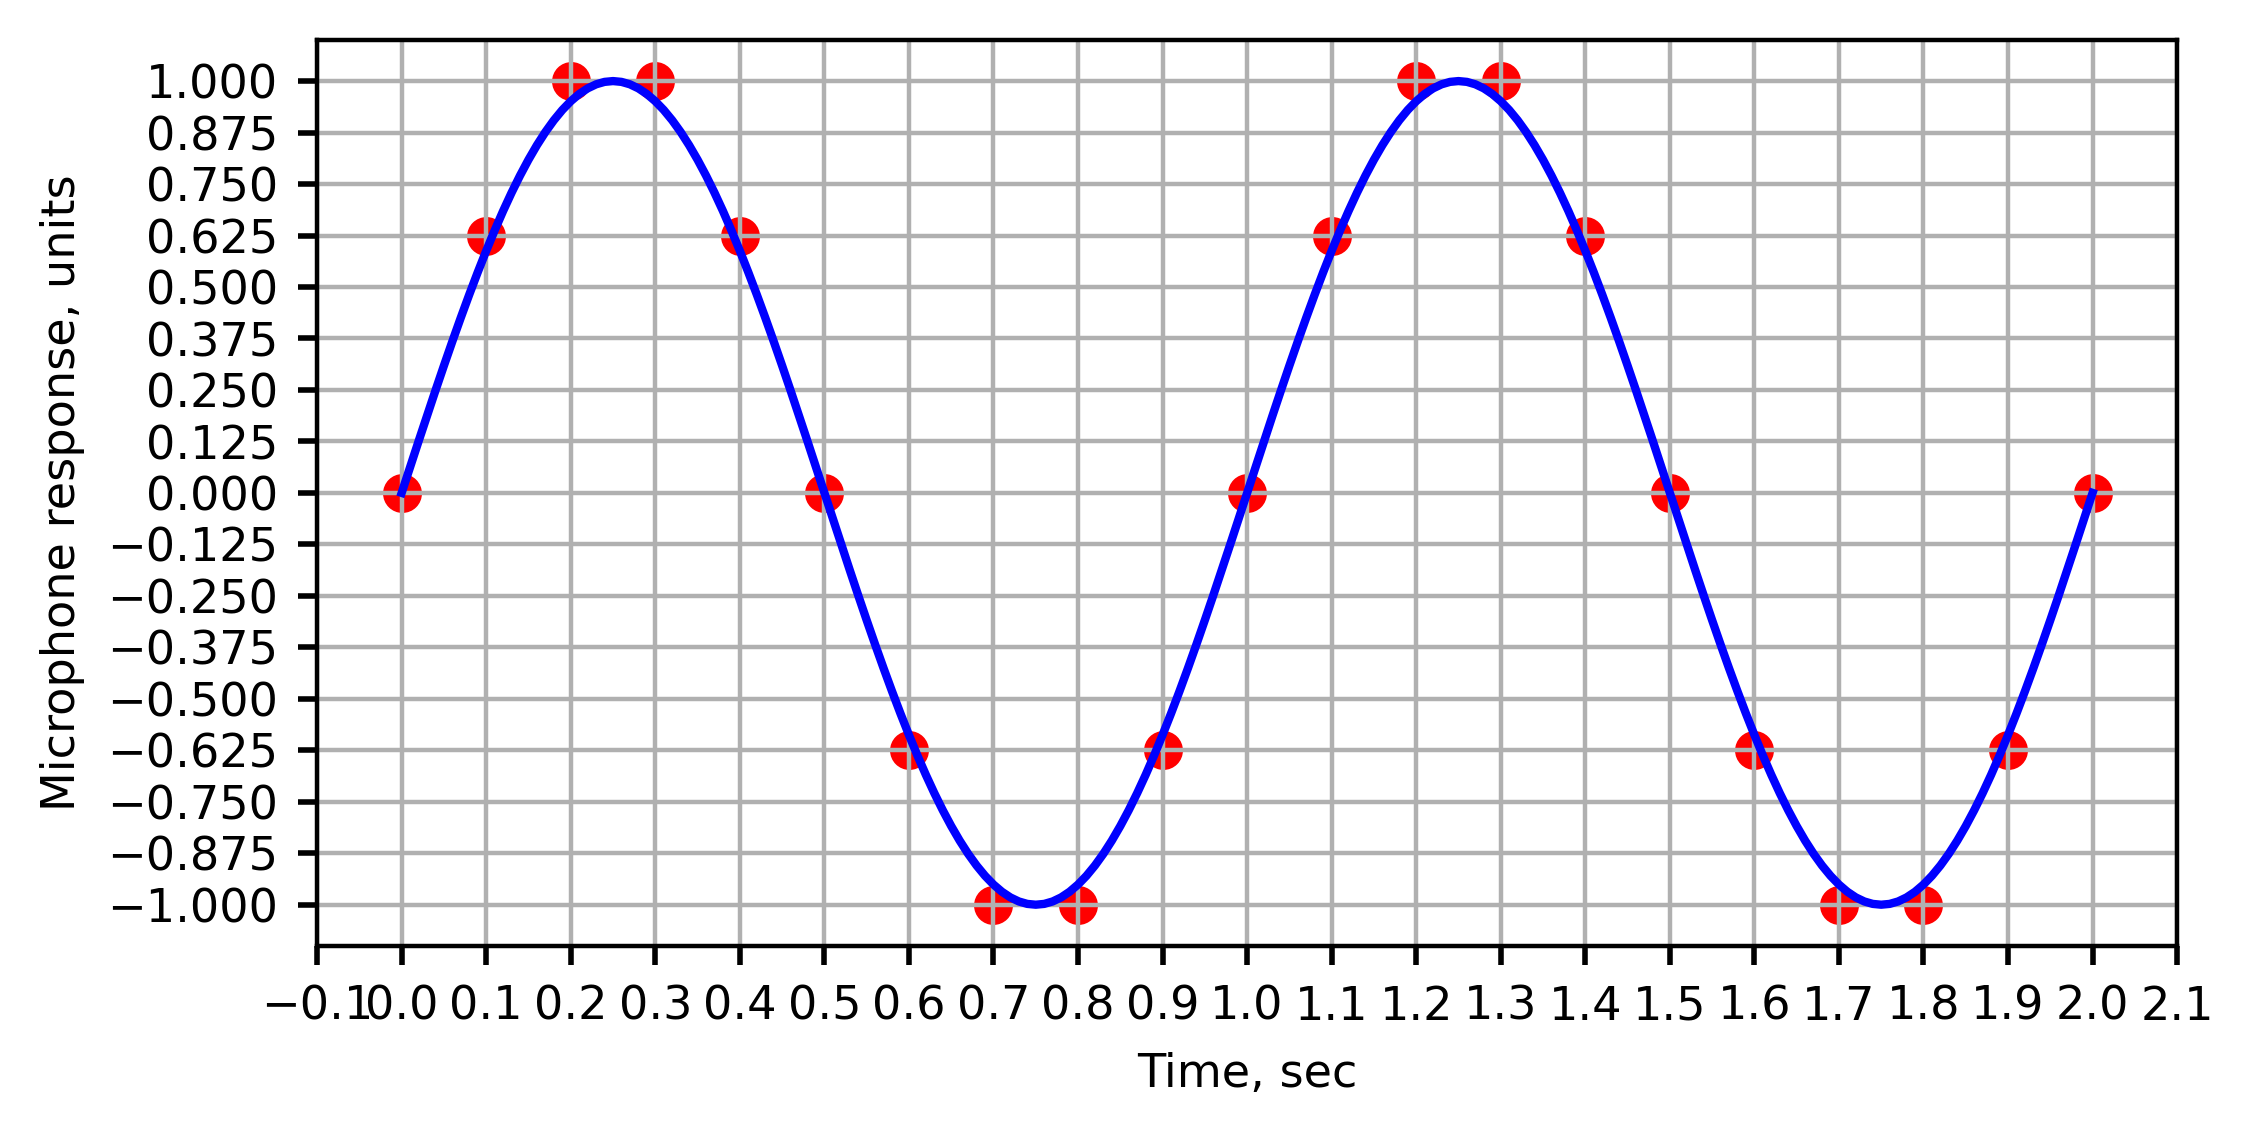
\includegraphics[width=1\linewidth]{\picPath/sound_discrete.png}
\end{center}
  \caption{Оцифровка синусоиды с частотой дискредитации 10Гц и глубиной 4 бита. Синим изображен исходный сигнал, красные точки - полученные в результате дискредитации значения.}
  \label{pic:wav_ex}
  \end{figure}


    Для извлечения входящих в звуковой сигнал базовых частот используется оконное дискретное преобразование Фурье, описанное в главе \ref{chap:Fourier}. Для визуализации базовых частот широко используются спектрограммы и MEL спектрограммы, описанные в главе \ref{chap:spectrogram}.

\section{Методы анализа звукового сигнала} 
\subsection{Преобразование Фурье}
\label{chap:Fourier}
Непрерывное преобразование Фурье имеет вид: 

Прямое:

$$
\begin{equation}
F(s) 
\equiv
\mathcal{F}\{f(x)\}(s)
\equiv
{\int\limits_{-\infty}^{\infty}f(x)\,e^{-2\pi i s x}\,dx~}
\end{equation}
$$

Обратное: 

$$
\begin{equation}
f(x) 
\equiv
\mathcal{F}^{-1}\{F(s)\}(x)
\equiv
{\int\limits_{-\infty}^{\infty}F(s)\,e^{2\pi i s x}\,ds~}
\end{equation}
$$

Где $f(x)$ - непрерывная функция - сигнал вещественной переменной,
$F(x)$ - непрерывная функция комплексной переменной - Фурье образ $f(x)$ \cite{Gonzalez}. 

Сверткой называют интегральное преобразование вида:
$$
\begin{equation}
(f*g)(x)
=
{\int\limits_{-\infty}^{\infty} f(y)\,g(x-y)\,dy~} 
=
{\int\limits_{-\infty}^{\infty} f(x-y)\,g(y)\,dy~}  
\end{equation}
$$

Корреляцией двух функций называют преобразование вида:
$$
\begin{equation}
(f \star g)(x) 
= 
{\int\limits_{-\infty}^{\infty} f(y)\,g(x+y)\,dy~} 
= 
{\int\limits_{-\infty}^{\infty} f(x+y)\,g(y)\,dy~}  
\end{equation}
$$

Для непрерывного преобразования Фурье доказана теорема свертки 

$$
\begin{equation}
{(f*g)(x)}
\equiv
\mathcal{F}^{-1} \{
\mathcal{F}(f) \cdot \mathcal{F}(g) 
\}
\label{correlation_theorem}
\end{equation}
$$

Аналогично теореме о свертке, существует теорема о корреляция

$$
\begin{equation}
{(f \star g)(x)} 
\equiv
\mathcal{F}^{-1} \{
\mathcal{F}^*(f) \cdot \mathcal{F}(g) 
\}
\end{equation}
$$

Где операция \hspace{3pt} $\cdot$ \hspace{3pt} $-$ скалярное произведение, а $\mathcal{F}^*(f)$ - комплексно сопряженный образ Фурье функции $f$ .

Представим звуковой сигнал как функцию $f(x)$, принимающую ненулевые значения в промежутке $(0, T)$,
значения $f(0) = \frac{\lim_{x \to +0}f(x)}{2}$  $f(T) = \frac{\lim_{x \to -T}f(x)}{2}$. Не каждая функция может быть представлена в частотном базисе путем преобразования Фурье, для этого должен быть выполнен ряд условий\cite{Gonzalez}. Поэтому также предположим, что $f(t)$ имеет непрерывный Фуьре образ $F(\mu)$, принимающий ненулевые значения только на отрезке $[-\mu_{max}, \mu_{max}]$ . 

Как было описано в главе \ref{chap:digital_repr}, во время записи звукового сигнала возможно сохранение только конченого числа точек во времени. Выбирая частоту дискретизации $\Delta T$, можно представить набор сэмплированных точек в виде:

$$
\begin{equation}
\tilde{f}(t) = 
f(t)s_{\varDelta T}(t)
=
\sum_{n = -\infty}^{\infty}
f(t)
\delta(t - n\varDelta T)
\end{equation}
$$

Где $\delta$ есть функция Дирака. Дискретная функция  $\tilde{f}(t)$ имеет Фурье образ $\tilde{F}(\mu)$

$$
\begin{equation}
\tilde{F}(\mu) = 
\frac{1}{\varDelta T}
\sum_{n = - \infty}^{\infty}
F(
\mu - \frac{n}{\varDelta T}
)
\label{Furier_sampling_result}
\end{equation}
$$

Из формулы видно, что $\tilde{F}(\mu)$ является непрерывной и периодической функцией с периодом $\frac{1}{\Delta T}$.
Из предположения о том, что ${F}(\mu)$ принимает ненулевые значения только на отрезке $[-\mu_{max}, \mu_{max}]$  и выбирая $\varDelta T = \frac{1}{2\mu_{max}}$, можем выразить  ${F}(\mu)$ из  $\tilde{F}(\mu)$ формулой:

$$
\begin{equation}
F(\mu)
=
H(\mu)
\tilde{F}(\mu)
\end{equation}
$$

Где 

$$
\begin{equation}
H(\mu)
=
\begin{cases}
\varDelta T & 
\mu \in [-\mu_{max},\mu_{max}] \\
0 & иначе
\end{cases}
\end{equation}
$$

Обратное преобразование Фурье для $H(\mu)$ имеет вид

\begin{gather*}
h(t)
=
\mathcal{F}^{-1}\{H(\mu)\}(t)
=
\int\limits_{-\infty}^{\infty}
H(\mu)
e^{2\pi i \mu t }
d\mu~
=
\int\limits_{-\mu_{max}}^{\mu_{max}}
\varDelta T
e^{2\pi i \mu t }
d\mu~
=
\\
=
\frac{\varDelta T}
{i 2 \pi t} 
\left[
e^{	2\pi i \mu t }
\right]_{-\mu_{max}}^{\mu_{max}}
=
2\varDelta T \mu_{max}
\frac{sin(2\pi t \mu_{max}) }{(2\pi t \mu_{max})}
=
2\varDelta T \mu_{max}
sinc(2t\mu_{max})
\end{gather*}

Тогда исходная функция $f(t)$ может быть получена из следующего соотношения:

\begin{gather*}
f(t)
=
\mathcal{F}^{-1}
\{ F(\mu) \}
\\
=
\mathcal{F}^{-1}
\{
H(\mu)\tilde{F}(\mu)
\}
\\
=
h(t)*\tilde{f}(t)
\end{gather*}

где последнее неравенство получено благодаря теореме свертки для пар образов Фурье. Соотношение можно переписать как

$$
\begin{equation}
f(t) 
=
\sum_{ n = - \infty}^{\infty}
f(n \varDelta T ) 
sinc[ (t - n \varDelta T) / \varDelta T	] 
=
\sum_{ n = 0}^{\frac{T}{\Delta T}}
f(n \varDelta T ) 
sinc[ (t - n \varDelta T) / \varDelta T	] 
\end{equation}
$$

Таким образом, выбирая частоту дискретизации  $\varDelta T = \frac{1}{2\mu_{max}}$, для сохранения непрерывной функции $f(t)$, удовлетворяющей всем заданным условиям, достаточно хранить $\frac{T}{\Delta T} + 1$ значений этой функции. Данный вывод называется теоремой Котельникова или сэмплирования.

$\tilde{F}(\mu)$ есть непрерывная ограниченная функция

$$
\begin{equation}
\tilde{F}(\mu)=\int_{-\infty}^{\infty} \tilde{f}(t) e^{-j 2 \pi \mu t} dt
\end{equation}
$$


$$
\begin{equation}
\begin{aligned}
\tilde{F}(\mu) &=\int_{-\infty}^{\infty} \tilde{f}(t) e^{-j 2 \pi \mu t} d t=\int_{-\infty}^{\infty} \sum_{n=-\infty}^{\infty} f(t) \delta(t-n \Delta T) e^{-j 2 \pi \mu t} d t \\
&=\sum_{n=-\infty}^{\infty} \int_{-\infty}^{\infty} f(t) \delta(t-n \Delta T) e^{-j 2 \pi \mu t} d t \\
&=\sum_{n=-\infty}^{\infty} f_{n} e^{-j 2 \pi \mu n \Delta T} =  \sum_{n=0}^{\frac{T}{\Delta T}} f_{n} e^{-j 2 \pi \mu n \Delta T}
\end{aligned}
\label{eq:discrete_image}
\end{equation}
$$


Для того, чтобы описать $\tilde{F}(\mu)$ достаточно сохранить всего $M=\frac{T}{\Delta T} + 1$ значений функции. Чтобы показать это, рассмотрим равномерную сетку частот

$$
\begin{equation}\mu=\frac{m}{M \Delta T} \quad m=0,1,2, \ldots, M-1 \label{freq_grid} \end{equation} 
$$

Принимая во внимание тот факт, что $\tilde{F}(\mu)$ периодическая с периодом $\Delta T$, что видно из формулы \ref{Furier_sampling_result}, достаточно сохранить значения только для одного из периодов этой функции. Тогда, подставляя \ref{freq_grid} в формулу \ref{eq:discrete_image},  получаем прямое дискретное преобразование Фурье:
\begin{equation}
F_{m}=\sum_{n=0}^{M - 1} f_{n} e^{-j 2 \pi m n / M} \quad m=0,1,2, \ldots, M-1
\label{FDFT}
\end{equation}

Обратное дискретное преобразование Фурье имеет вид
\begin{equation}
f_{n}=\frac{1}{M} \sum_{m=0}^{M-1} F_{m} e^{j 2 \pi m n / M} \quad n=0,1,2, \ldots, M - 1
\label{BDFT}
\end{equation}

Можно показать, что при подстановке \ref{FDFT} в \ref{BDFT} можно получить равенство $f_n = f_n$, аналогично, подставляя \ref{BDFT} в \ref{FDFT} можно получить равенство $F_m = F_m$. Таким образом последовательности $\{f_m\}$ взамиооднозначно ставиться в соответствие последовательность образов $\{F_m\}$.  Если частота дискретизации исходного сигнала равна $\Delta T$, то шаг сетки частот будет равен $\Delta \mu = \frac{1}{M \Delta T}   = \frac{1}{T + \Delta T}$ 

Для случая дискретного преобразования Фурье, также как и для непрерывного случая, действует теорема свертки\cite{bib:bio_signals_and_image_proc}, позволяющая улучшить асимптотику операций свертки и кросс корреляции используя для этого переход в частотный базис.

 Последовательность $\{F_m\}$ есть комплексные коэффициенты дискретного ряда Фурье. Переходя в полярные координаты $F_m = F^r_m + j \cdot F^j_m = \mid F_m \mid \cdot e^{j \theta_m}$ , можно представить прямое дискретное преобразование Фурье следующим образом: 

$$
\begin{equation}
\begin{aligned}
f_{n}=\frac{1}{M} \sum_{m=0}^{M-1} F_{m} e^{j 2 \pi m n / M} 
=
\frac{1}{M} \sum_{m=0}^{M-1} \mid F_m \mid \cdot e^{j \theta_m} \cdot  e^{j 2 \pi m n / M}  
\\=
\frac{1}{M} \sum_{m=0}^{M-1} \mid F_m \mid  \cdot  e^{j( 2 \pi m n / M + \theta_m)} \quad
\end{aligned}
\end{equation}
$$

$$
e^{j(\omega \cdot n + \theta_m)} = \sin(\omega \cdot n + \theta_m) + j\cos(\omega \cdot n + \theta_m)
$$
Из равенства видно, что $\mid F_m \mid$ отвечают за магнитуду, входимую в исходный сигнал соответствующей базовой частоты, и $\theta_m$ отвечает за сдвиг этой базовой частоты или фазу.

На практике для частотного анализа сигналов их разбивают на отдельные части - окна, для каждого из которых находятся коэффициенты ряда Фурье. Последовательность полученных коэффициентов используется как приближение разложения в ряд Фурье всей последовательности. 

Оконное дискретное преобразование Фурье (Short Time Discrete Fourier Transformation)\cite{bib:bio_signals_and_image_proc} определяется как 

$$
\begin{equation}
\operatorname{STFT}\{f(n)\}(m_k, \omega) \equiv F(m_k, \omega)=\sum_{n=0}^{M-1} f(n) w(n-m_k) e^{-j \omega n}
\end{equation}
$$

где $f(n)$ - исходный дискретный сигнал, $w(n)$ - оконная функция, $m_k$ - последовательность сдвигов оконной функции.

\subsection{Спектрограмма и её разновидности}
\label{chap:spectrogram}
Спектрограмма или магнитудная спектрограмма — это визуальное представление спектра частот сигнала, меняющегося во времени\cite{bib:think_DSP}, определяется как 

$$
\begin{equation}
\operatorname{spectrogram}(t, \omega)=|\operatorname{STFT}(t, \omega)|^{2}
\end{equation}
$$


\begin{figure}[H]
\begin{center}
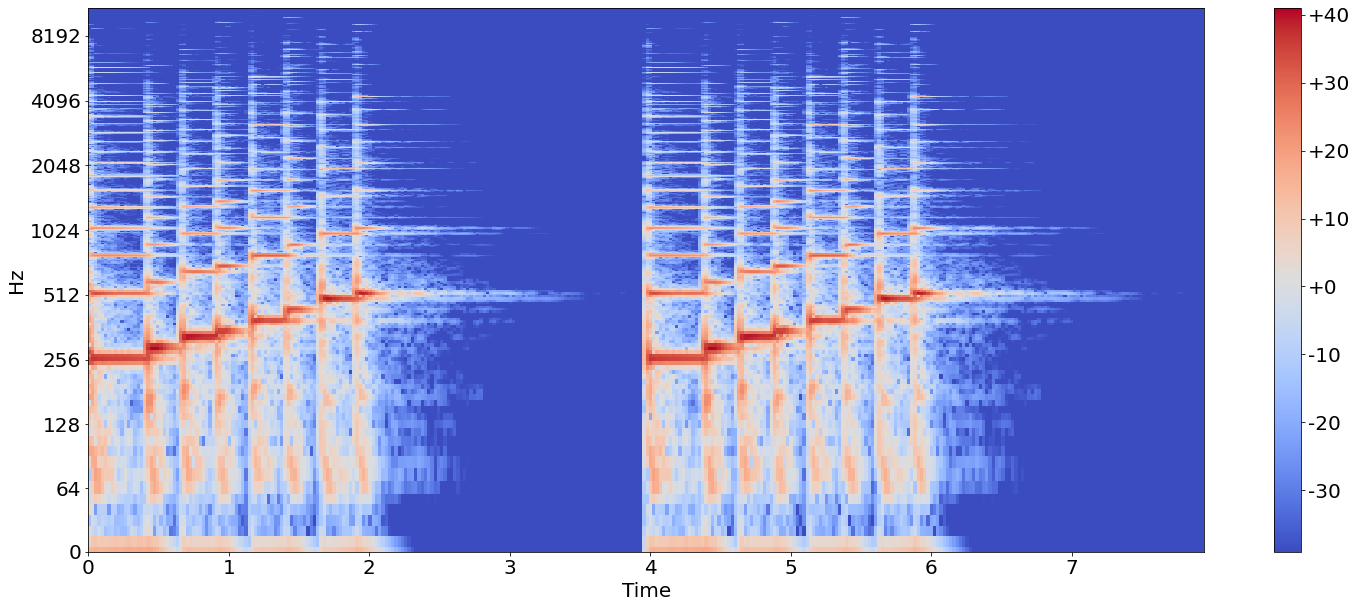
\includegraphics[width=1\linewidth]{\picPath/spectrogram.png}
\end{center}
  \caption{Пример магнитудной спектрограммы аудиозаписи фортепиано}
\end{figure}



Как видно из формулы, спектрограмма сохраняет только магнитуды базовых частот, не учитывая влияние сдвига для каждой базовой частоты. Спектрограмму можно представить в виде матрицы $S_{M \times W}$ где $M$ - количество частот в дискретном разложении Фурье и $W$ - количество окон, необходимое для покрытия данного на вход файла. Такое упрощенное представление позволяет визуализировать распределение магнитуд частот исходного сигнала и упрощает его обработку. Недостаток использования такого подхода обработки сигналов - невозможность точного обратного преобразования спектрограммы в исходный сигнал.

Стандартным способом представления звуковых сигналов  является MEL- спектрограмма\cite{bib:librosa}. Популярность этого метода обусловлена тем, что MEL базис отражает восприимчивость человеческого уха на частоты определенной высоты: из экспериментов обнаружено, что низкие звуковые частоты человеческий слух отличает лучше, чем высокие. Базис MEL частот выражается следующей формулой: 

$$
\begin{equation}
\operatorname{Mel}(f)=2595 \log _{10}\left(1+\frac{f}{700}\right)
\end{equation}
$$

Для того, чтобы посчитать MEL спектрограмму на основе магнитудной спектрограммы, необходимо сперва вычислить Filter bank - матрицу коэффициентов для фильтрации исходного частотного представления сигнала\cite{bib:librosa}. Первоначально задается параметр - количество фильтров $P$. В частотном базисе равномерно относительно MEL шкалы определяется сетка из точек, количество которых равно количеству фильтров. Как видно на рисунке \ref{pic:filter_bank}, каждому фильтру соответствует точка в сетке, в которой значение фильтра равно 1. Проводятся две прямые: из предыдущей точки сетки в текущую и из текущей точки в следующую, при этом в соседних точках фильтр принимает значение 0.


\begin{figure}[H]
\begin{center}
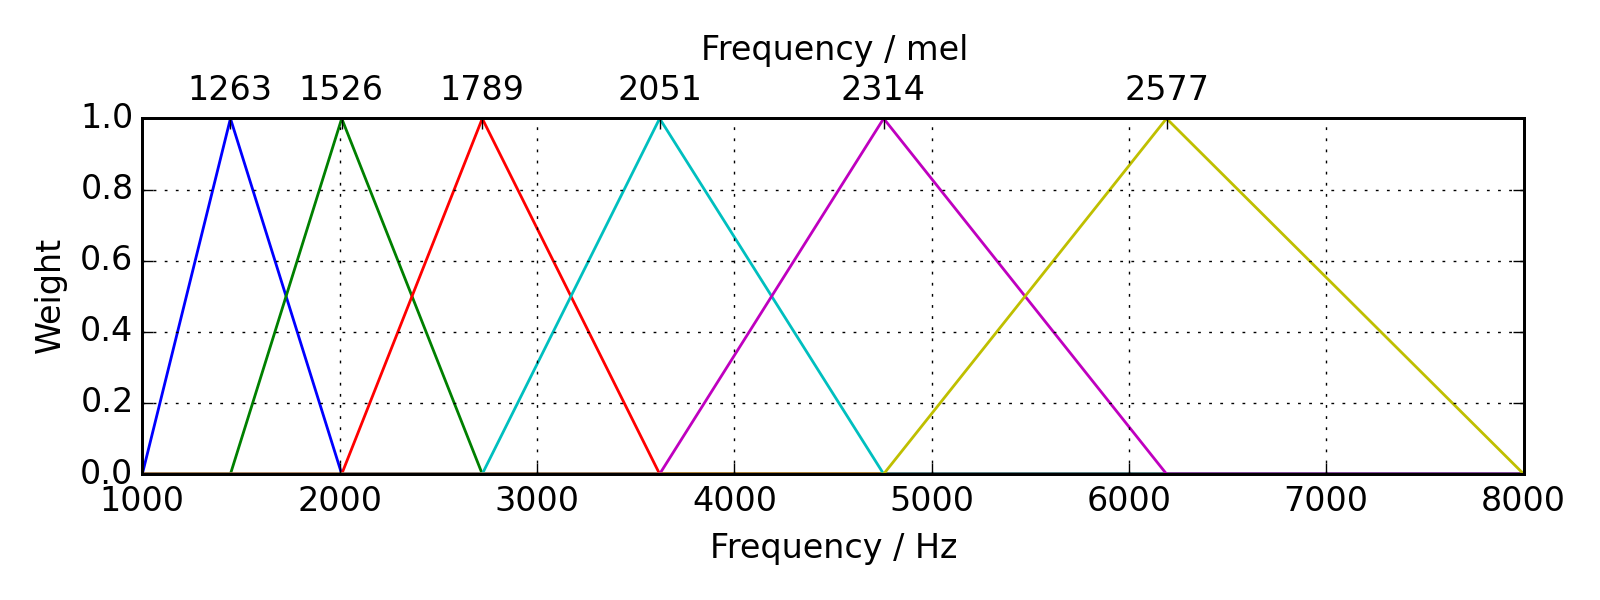
\includegraphics[width=1\linewidth]{\picPath/filter_bank.png}
\end{center}
  \caption{Пример Filter bank для $P = 6$}
  \label{pic:filter_bank}
  \end{figure}


Полученный фильтр - матрица коэффициентов  $\text{filter}_{P \times M}$, в каждой строчке содержит соответствующий фильтр для определенной частоты, в то время как  магнитудная спектрограмма $S_{M \times W }$ в каждом столбце содержит значения магнитуд базовых частот для соответствующих окон. Фильтр применяется к спектрограмме следующим образом:

$$
\begin{equation}
\text{Mel} = filter \times S
\end{equation}
$$

Результат применения такого фильтра -  матрица размерности $M \times W$ - MEL коэффициенты для каждого из окон спектрограммы


Другой способ представления сигналов - мел-кепстральные коэффициенты (Mel-frequency cepstral coefficients - MFCC)\cite{bib:librosa}\cite{bib:MFCC}\cite{bib:MFCC_choice}


$$
\begin{equation}
\mathrm{MFCC}_{i}=\sum_{k=0}^{P-1} \text{Mel}[k,:] \cos \left[i\left(k-\frac{1}{2}\right) \frac{\pi}{P}\right], \quad i=1,2, \cdots, M_{MFCC}
\end{equation}
$$

Матрица $\mathrm{MFCC}_{ M_{MFCC} \times W }$ получается из MEL спектрограммы путем применения к ней косинусного преобразования\cite{bib:MFCC_choice}



\chapter{Клонирование голоса}
\section{Постановка задачи}
\label{chap:task_def}
Дан короткий звуковой файл длиной 5-10 секунд, необходимо преобразовать текст на русском языке в голос так, как если бы этот текст читал человек, записанный на входном звуковом сигнале. Задача дополняет проблему генерации голоса по тексту (Text To Speech, TTS) условием схожести выходного голоса с голосом, переданным на вход. 

Датасеты для решение задачи клонирования голоса представляют из себя такие признаки как:

\begin{itemize}
\item номер (id) спикера;
\item аудиозапись длинной 3-10 секунд;
\item текстовая расшифровка аудиозаписи.
\end{itemize} 

Автор работы \cite{bib:voice_cloning} предлагает разбиение задачи клонирования голоса на 2 подзадачи:
1) Идентификация спикера по голосу
2) Условная генерация голоса по тексту

Для того, чтобы параметризовать задачу генерации голоса, автор предлагает использовать закодированное представление спикера из задачи идентификации, которое используется как дополнительный признак генеративной модели.

Популярный тренд развития области TTS - разбиение моделей генерации на две части: предсказание MEL-спектрограммы и предсказание непосредственно звукового сигнала на основе полученной MEL спектрограммы.

Существует известнае модификации репозитория \cite{bib:voice_cloning}, автор которого попытался решить поставленную задачу для русского языка\cite{bib:russian_voice_cloning}, однако результаты работы субъективно уступают качеству английской версии модели. Возможные причины субъективно низкого качества генерации - чрезмерное усложнение модели, приводящее к переобучению на небольшом тренировочном наборе и использование тренировочных данных низкого разрешения, что может привести к переобучению блока генерации речи (TTS) на имеющиеся в датасете искажения и шумы.

В рамках работы предлагается использовать оригинальную архитектуру моделей из репозитория Voice Cloning\cite{bib:voice_cloning} и выбрать для тренировки датасеты с аудиозаписями высокого разрешения. Подробности выбора данных описаны в главе \ref{chap:data}.

К сожалению, на сегодняшний день не существует объективной метрики оценки качества генерации голоса кроме только значения функции ошибки \cite{bib:voice_cloning}, поэтому для валидации работы используется субъективная метрика "Средняя оценка эксперта (Mean Option Score)" .
\section{Связанные задачи}
\subsection{Задача идентификация спикера}

Даны набор аудиозаписей, на которых записаны голоса разных спикеров, причем в каждой аудиозаписи присутствует голос только одного спикера. Необходимо разметить аудиозаписи так, чтобы каждый элемент набора получил метку, причем записи, произведенные одним спикером, должны иметь одинаковую метку, а записи, произведенные разными спикерами - разные.

Для решения данной задачи хорошо зарекомендовал себя подход, основанный на моделях LSTM \cite{bib:lstm} и обобщенной функции ошибки для задачи верификации спикера (Generalized End to End Loss, GE2E)\cite{bib:e2e_speaker_ver_loss}.

В качестве признаков используются MEL-спектрограммы, полученные из входных аудиозаписей. Элементы датасета имеют вид $\{\mathbf{x}_{j,i}\}$, где $j$  есть индекс спикера, а $i$ есть индекс фразы этого спикера. GE2E подход появился как улучшение предшествующего метода - Tuple Based End to End Loss (TE2E), суть которого заключается в следующем: входные признаки делятся на пары $\left\{\mathbf{x}_{j \sim},\left(\mathbf{x}_{k 1}, \ldots, \mathbf{x}_{k M}\right)\right\}$.
Первый элемент и $M$ элементов второго элемента пары преобразовываются в латентное пространство посредством LSTM модели \cite{bib:lstm} и нормированием по L2 норме в пару вида $\left\{\mathbf{e}_{j \sim},\left(\mathbf{e}_{k 1}, \ldots, \mathbf{e}_{k M}\right)\right\}$. Для того, чтобы сравнить вектор спикера $j$ со всеми векторами спикера $k$, набор $\left(\mathbf{e}_{k 1}, \ldots, \mathbf{e}_{k M}\right)$ агрегируется посредством поэлементного усреднения:

$$
\begin{equation}
\mathbf{c}_{k}=\mathbb{E}_{m}\left[\mathbf{e}_{k m}\right]=\frac{1}{M} \sum_{m=1}^{M} \mathbf{e}_{k m}
\end{equation}
$$

Значение $\mathbf{c_k}$ называется центроидом спикера $k$. Вычисляя схожесть векторов $\mathbf{x}_{j \sim}$ и $\mathbf{c}_{k}$ при помощи косинусного расстояния с обучающимися парамметрами $w$ и $b$ 

$$
\begin{equation}
s=w \cdot \cos \left(\mathbf{e}_{j \sim}, \mathbf{c}_{k}\right)+b
\end{equation}
$$

итоговая функция ошибки для сети выглядит следующим образом:

$$
\begin{equation}
L_{\mathrm{T}}\left(\mathbf{e}_{j \sim}, \mathbf{c}_{k}\right)=\delta(j, k)(1-\sigma(s))+(1-\delta(j, k)) \sigma(s)
\end{equation}
$$

В качестве альтернативы авторы \cite{bib:e2e_speaker_ver_loss} предложили сравнивать не только один признак $j$ спикера, но сравнивать сразу $N$ спикеров, каждый из которых имеет $M$ фраз, друг с другом попарно. Для этого исходный набор признаков $\{\mathbf{X}_{j , i}\}, j = 1\cdots N, i=1\cdots M$ транслируется в латентное пространство при помощи LSTM модели: 

$$
\begin{equation}
\mathbf{e}_{j i}=\frac{f\left(\mathbf{x}_{j i} ; \mathbf{w}\right)}{\left\|f\left(\mathbf{x}_{j i} ; \mathbf{w}\right)\right\|_{2}}
\end{equation}
$$

где $f$ - функция модели LSTM, а $\mathbf{w}$ - её веса. Затем, также с использованием обучаемых параметров $w$  и $b$, вычисляется тензор схожести $\mathbf{S}_{j i, k}$:



\begin{equation}
\mathbf{S}_{j i, k}= \begin{cases}w \cdot \cos \left(\mathbf{e}_{j i}, \mathbf{c}_{j}^{(-i)}\right)+b & \text { if } \quad k=j \\ w \cdot \cos \left(\mathbf{e}_{j i}, \mathbf{c}_{k}\right)+b & \text { otherwise }\end{cases}
\end{equation}

\begin{equation}
\mathbf{c}_{j}^{(-i)}=\frac{1}{M-1} \sum_{\substack{m=1 \\ m \neq i}}^{M} \mathbf{e}_{j m}
\end{equation}


Элемент тензора $ji,k$ отвечает за схожесть $i$ фразы $j$ спикера с центроидом спикера $k$. Для того, чтобы непосредственно посчитать функцию ошибки, авторы\cite{bib:e2e_speaker_ver_loss} предлагают два возможных подхода:
Softmax:

\begin{equation}
L\left(\mathbf{e}_{j i}\right)=-\mathbf{S}_{j i, j}+\log \sum_{k=1}^{N} \exp \left(\mathbf{S}_{j i, k}\right)
\end{equation}
Контрастная функция ошибки:

\begin{equation}
L\left(\mathbf{e}_{j i}\right)=1-\sigma\left(\mathbf{S}_{j i, j}\right)+\max _{\substack{1 \leq k \leq N \\ k \neq j}} \sigma\left(\mathbf{S}_{j i, k}\right)
\end{equation}
Итоговое значение ошибки для всего тензора схожести определяется так:
$$
\begin{equation}
L_{G}(\mathbf{x} ; \mathbf{w})=L_{G}(\mathbf{S})=\sum_{j, i} L\left(\mathbf{e}_{j i}\right)
\end{equation}
$$

В случае функции ошибки типа Softmax, чем больше вектора, относящиеся к разным спикерам, больше похожи друг на друга, тем больше ошибка. Но так как задача, кроме всего прочего, требует, чтобы вектора одного спикера были похожи друг на друга - из суммы вычитается значение $\mathbf{S}_{j i, j}$. Так как производная нового отрицательного слагаемого, начиная с некоторого момента, больше, чем доля, вносимая  $\mathbf{S}_{j i, j}$ в сумму логарифмов - можно сказать, что ошибка тем больше, чем ближе вектора разных спикеров и тем меньше, чем ближе вектора одного и того же спикера. То же самое можно сказать о контрастной версии ошибки для данной задачи.

Сравнивая GE2E  и TE2E подходы, авторы приводят следующие аргументы в пользу обновленной версии: во время вычисления $L(\mathbf{e}_{ij})$ в GE2E используется $N \times M$ векторов спикеров одновременно, что приводит к тому, что во время обратного распространения ошибки путем градиентного спуска все $N \times M $ векторов стремятся в желаемом направлении: вектора одного спикера сжимаются в кластер, а разных спикеров - отдаляются. В то время как аналогичный шаг в TE2E задействует только лишь $M + 1$ вектор. Таким образом, можно ожидать, что подтверждается экспериментами, что модель сходится к лучшему результату за меньшее число шагов тренировки.


\subsection{Задача преобразование текста в речь}
Дан текст на естественном языке. Необходимо сгенерировать аудиозапись, содержащую человеческую речь, воспроизводящую данный на вход текст.  Задача входит в класс проблем трансляции последовательности (текст) в последовательность (аудиозапись) (Sequence to Sequence). 

Часто используемый метод решения данной задачи - модель Tacotron\cite{bib:Tacotron}, имеющая на данный момент две версии реализации. Модель состоит из энкодера текcта(encoder), блока внимания (attention block) и декодера(decoder), который генерирует непосредственно столбцы MEL спектрограммы. Схему архитектуры модели изображена на рисунке\ref{pic:Tacotron}

Первая подзадача - транслирование текста на естественном языке в репрезентативное латентное пространство, для чего используется блок-энкодер. В качестве входных элементов используются отдельные символы, которые при помощи операции embedding\cite{bib:pytorch} преобразовываются в вещественные вектора. Далее к каждому полученному вектору поэлементно применяется нелинейная операция - dropout\cite{bib:pytorch}.  После этого набор векторов передается в подсеть CBHG. 

Первый этап подсети CBHG - свертка входной последовательности с набором конволюций $C_k, k=1 \cdots K$, где $C_k$ есть одномерная конволюция с ядром размерности $k$. Параметр stride конволюций равен 1, поэтому на выходе этого блока для каждого символа строится $K$ векторов, из которых затем путем применения операции max pooling для каждого входного символа выбирается наибольшее по модулю значение сверток. Таким образом, после прохождения блока наборов конволюций выход модели для каждого из элементов обладает контекстной информацией.

\begin{figure}[H]
\begin{center}
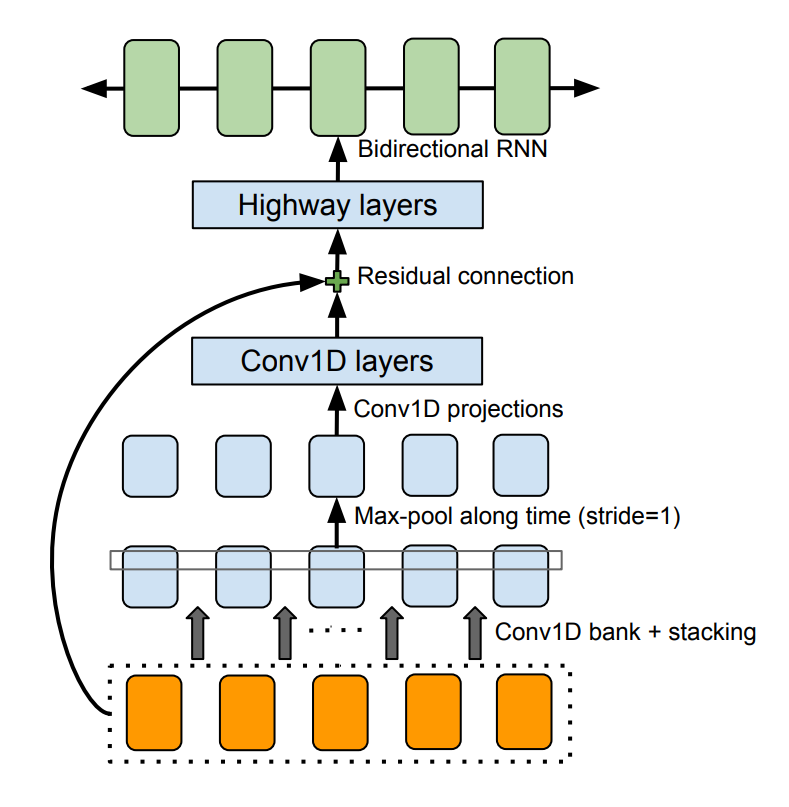
\includegraphics[width=0.7\linewidth]{\picPath/CBHG.png}
\end{center}
  \caption{Архитектура блока CBHG}
  \label{pic:CBHG}
  \end{figure}


После операции max pooling к последовательности применяется несколько одномерных конволюций с фиксированной размерностью фильтров, и входная последовательность складывается полученной последовательностью векторов, что называется residual connection, что позволяет улучшить сходимость модели благодаря уменьшению влияния проблему резкого роста / затухания градиента\cite{bib:resnet}.

Далее к полученному вектору применяется блок, называемый highway networks \cite{bib:highway_net}, который можно описать следующим образом:

\begin{equation}
\mathbf{y}=H\left(\mathbf{x}, \mathbf{W}_{\mathbf{H}}\right) \cdot T\left(\mathbf{x}, \mathbf{W}_{\mathbf{T}}\right)+\mathbf{x} \cdot\left(1-T\left(\mathbf{x}, \mathbf{W}_{\mathbf{T}}\right)\right)
\end{equation}

где $x$ и $y$ - входы и выходы блока соответственно, $\mathbf{H}$ есть основная операция блока c параметрами $\mathbf{W}_{\mathbf{H}}$ и блок переноса (carry) $T$ с параметрами $\mathbf{W}_{\mathbf{T}}$. Мотивация highway network блока - возможность роста значения градиента по пути переноса carry, способствующая уменьшению вероятность затухания / резкого роста градиента \cite{bib:highway_net}.  

После этого к последовательности применяется блок двусторонней рекурентной сети GRU\cite{bib:GRU},  позволяющий представить всю данную на вход последовательность, которая может иметь произвольную длину, в виде вектора фиксированной размерности. Главное отличие рекуррентных сетей от остальных - хранение состояния. Рекуррентные сети имеют два входа и два выхода - входы / выходы для состояния модели и входы / выходы для векторов латентного пространства. На первом этапе работы блоку передается первый элемент последовательности на вход для латентных векторов и начальное состояние блока на вход состояния. На втором этапе работы на вход для латентных векторов передается второй элемент входной последовательности, но при этом на вход состояния передается выход состояния блока на предыдущем этапе. На последнем этапе последний элемент входной последовательности обрабатывается рекуррентной сетью с учетом всех предыдущих этапов, и выходной латентный вектор используется как выход всего блока. Подробное устройство блока GRU можно найти в работе авторов\cite{bib:GRU}. После каждой операции свертки в сети, для улучшения сходимости, используется операция batchnorm\cite{bib:pytorch}.

Таким образом определяется блок энкодера, который преобразует наборы символов в вектор фиксированной длины, содержащий внутри некоторое представление входных данных с учетом контекстной информации. 

\begin{figure}[H]
\begin{center}
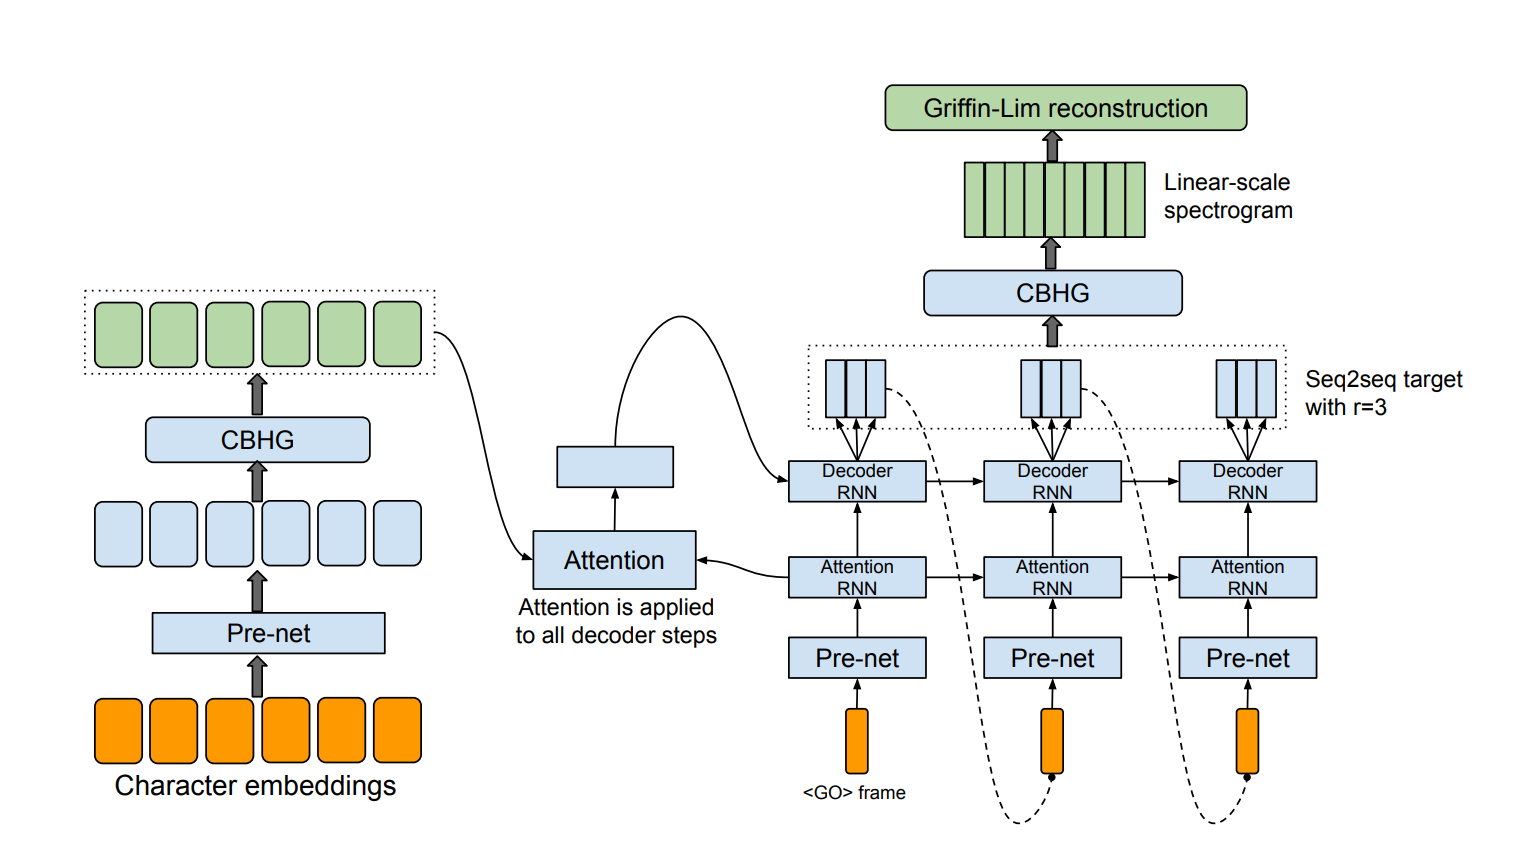
\includegraphics[width=1\linewidth]{\picPath/Tacotron.png}
\end{center}
  \caption{Архитектура TTS модели Tacotron}
  \label{pic:Tacotron}
  \end{figure}
  
  В качестве блока внимания (attantion) использовался блок, основанный на функции tanh \cite{bib:attention}, который можно описать формулой \ref{eq:attn}: 
  
  $$
  \begin{equation}
 \text{attn}(\mathbf{q}, \text{enc}) = \text{softmax} (\mathbf{V}\cdot\tanh(\mathbf{W} \cdot \mathbf{q} + \text{enc} ))
 \label{eq:attn}
  \end{equation}
  $$
  
  где $\mathbf{V}, \mathbf{W}$ - матрицы обучаемых параметров, которые кроме того могут быть использованы для того, чтобы размености входного вектора  $\mathbf{q}$  и выхода $\text{attn}$ совпадали.  $\text{enc}$ - выход блока энкодера. Блок внимания используется для того, чтобы учесть текстовую информацию во время генерации звукового сигнала. Природа параметра $\mathbf{q}$ (query) зависит от задачи, и в данном случае является состоянием блока декодера.
  
  Блок декодера генерирует выход модели - MEL спектрограмму. В качестве целевых параметров была выбрана MEL спектрограмма с 80 bank фильтрами.  Декодер состоит из нелинейного блока, аналогичного с нелинейным блоком в энкодере, блока внимания, двух рекуррентных блоков и блока последнего линейного слоя, который непосредственно предсказывает матрицу спектрограммы и присоединен к последнему рекуррентному блоку. 
  
  Работа декодера происходит следующим образом: в первый нелинейный блок декодера на вход на первом этапе передается начальный вектор <go>, вместо которого на следующих этапах используется предыдущее состояние выхода декодера.  Нелинейный блок затем передает свой выход в первый рекуррентный блок GRU, выходы которого передаются на вход в блок внимания и рекуррентный блок LSTM\cite{bib:LSTM}; блок LSTM принимает на вход результат операции внимания и выход блока GRU, выдавая на выходе столбцы результирующей MEL-спектрограммы. Так как соседствующие столбцы MEL-спектрограммы сильно коррелируют друг с другом, авторы предлагают генерировать сразу $r$ столбцов матрицы и использовать в качестве состояния декодера последний $r-1$ столбец. В оригинальной модели гиперпараметр $r = 3$. Стоит заметить, что во время тренировки используется подход Teacher forcing\cite{bib:teacher_forcing}, принцип которого заключается в том, что во время тренировки вместо передачи генерированного на прошлом этапе столбца спектрограммы, в модель передается соответствующий столбец из Mel-спектрограммы - желаемого выхода модели, что позволяет упростить и ускорить тренировку рекурентных моделей.  
  
  Как видно из рисунка \ref{pic:Tacotron}, после последнего линейного слоя может быть добавлен вспомогательный блок CBHG, однако в работе о клоноровании голоса\cite{bib:voice_cloning} этот блок не используется.
  
  Таким образом, описанная выше архитектура позволяет при помощи датасета типа текст-речь получить предсказание MEL спектрограммы. Для парамметризации модели на векторах, описывающих спикеров, эти вектора конкатинируются с каждым эмбеддингом выхода энкодера модели Tacotron. Таким образом модель понимает, когда от нее требуется воспроизвести текст выбранным способом. Предполагается, что с большим количеством тренировочных данных модель синтеза речи сможет генерализовать представление спикера и научиться генерировать голос новых, незнакомых, но похожих на спикеров из тренировочной выборки, спикеров.
  
\subsection{Задача восстановления звукового сигнала из MEL-спектрограммы}

Последний этап генерации голоса на основе тексте - восстановление звукового сигнала на основе MEL-спектрограммы. 

Во время трансляции звукового сигнала в MEL спектрограмму методом FFT, часть данных, а именно мнимые коэффициенты ряда Фурье, отвечающие за сдвиг базового сигнала то есть фазу - стираются. Задача заключается в восстановлении закодированного в MEL спектрограмму звукового сигнала в первоначальный базис. У этой задачи есть классический алгоритм решения - алгоритм реконструкции Гриффина-Лимма \cite{bib:phase_estim}.  Однако на практике алгоритм Гриффина-Лима превносит значительные для слуха артефакты в раскодированный аудио сигнал. Популярный метод решения - использования нейронных сетей. В работе по клонированию \cite{bib:voice_cloning} для реконструкции фазовой информации спектрограмм используется архитектура waveRNN\cite{bib:waveRNN}.
Модель waveRNN основывается на своем предшественнике - модели wavenet\cite{bib:wawnet}, которая моделирует закодированный аудиосигнал $\{x_1, \cdots ,x_T\}$ как совместное распределение:  

$$
\begin{equation}
p(\mathbf{x})=\prod_{t=1}^{T} p\left(x_{t} \mid x_{1}, \ldots, x_{t-1}\right)
\end{equation}
$$

В каждом блоке модели используется одномерные конволюции с параметрами $\text{dilate} = 1, 2, 4, \cdots, 2^N$. где $N$ - количество блоков в модели. Такой набор параметров позволяет увеличить рецептивное поле модели, не увеличивая при этом количество вычислений\cite{bib:wavenet}. Один блок модели wavenet можно описать следующей формулой:

$$
\begin{equation}
\mathbf{z}(\mathbf{x})= W_k \cdot\tanh \left(W_{f, k} * \mathbf{x}\right) \odot \sigma\left(W_{g, k} * \mathbf{x}\right)
\end{equation}
$$

где $\mathbf{x}$ - вход слоя, $k$ - индекс слоя, $W$ обучаемые параметры, $*$ - операция свертки, $\odot$ - символ поэлементного умножения, $\cdot$ - символ скалярного умножения, $V$ - матрица локального контекста, $\mathbf{h}$ - вектор глобального контекста. Индекс $f$ символизирует, что параметры относятся к основному пути вычислений модели, и $g$ значит, что веса относятся к дополнительной ветке модели, добавленной для ускорения сходимости тренировки модели. Как утверждают авторы, такая архитектура блока тренируется лучше, чем архитектура без дополнительной "gate" ветки вычислений\cite{bib:wawenet}.  Для ускорения обучения каждый блок имеет resudual connection связь, которая складывает результат вычисления блока с входом этого блока:

$$
\begin{equation}
\mathbf{Z}_{\text{skip}}(\mathbf{x})= \mathbf{z}(\mathbf{x}) + \mathbf{x}
\end{equation}
$$

 где $+$ - поэлементное сложение. Кроме того, для ускорения обучения также используется skip connection - выход каждого блока, прежде чем передаваться в последний этап обработки в модели, складывается друг с другом посредством полементного сложения. Послединй этап обработки модели есть парой последовательность операций Relu- одномерная конволюция с ядром размерности 1 и операцией softmax на выходе.  Архитектура всей модели изображена на рисунке \ref{pic:wavenet}.
 
 
 \begin{figure}[H]
\begin{center}
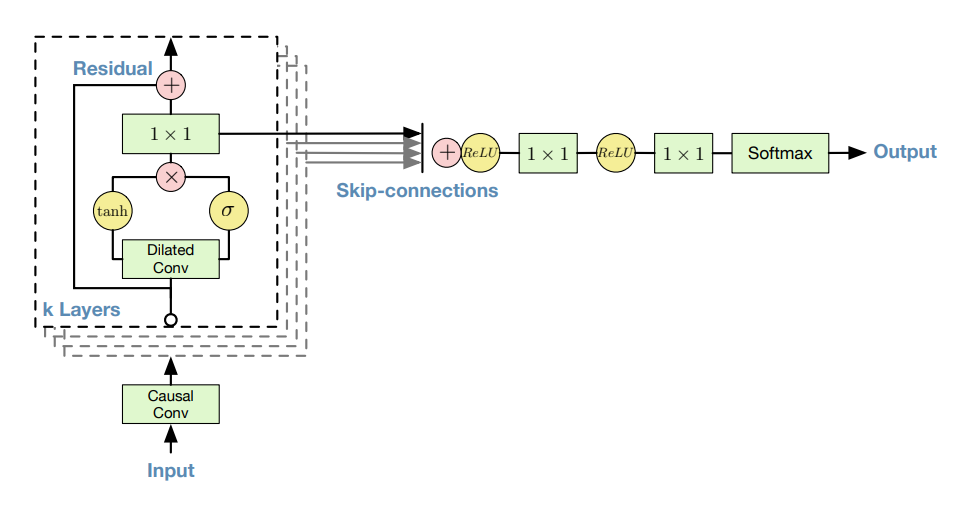
\includegraphics[width=1\linewidth]{\picPath/wavenet.png}
\end{center}
  \caption{Архитектура модели Wavenet}
  \label{pic:wavenet}
  \end{figure}
  
  Благодаря своей архитектуре во время тренировки с использованием подхода teacher forcing \cite{bib:teacher_forcing} предсказание каждого элемента выходного сигнала может быть произведено независимо друг от друга, что позволяет тренировать модель в распределенном режиме\cite{bib:wavenet}. Однако, в свою очередь, такой подход замедляет работу модели в режиме инференса: для генерации каждого последующего элемента выхода модели требуется все предыдущие, что не позволяет производить инференс модели в параллельном режиме. Кроме того, полученная архитектура имеет достаточно высокую вычислительную сложность. 
  
  Следующая версия модели - WaweRNN \cite{bib:waveRNN} не имеет недостатков, упомянутых выше, благодаря модифицированной архитектуре модели. WaveRNN состоит из одного рекуррентного блока и использует subscaling алгоритм для ускорения генерации выходного сигнала.
  
Пусть входная спектрограмма $\mathbf{u}$ проецируется в набор элементов $u = P(\mathbf{u})$. Входная последовательность $\mathbf{u}$ разбивается на $B$ подпоследовательностей длиной $\frac{\|\mathbf{u}\|}{B}$. Каждая подпоследовательность с индексом $i$ содержит элементы из $\mathbf{u}$ с индексами $i + kB, k =0 \cdots \frac{\| \mathbf{u} \|}{B}$. Обозначение $u_{i + j}$ значит, что это элемент $j$ подпоследовательности с индексом $i$. Тогда алгоритм subscaling можно описать следующей формулой:


\begin{equation}
\begin{array}{r}
P(\mathbf{u})=\prod_{s=0}^{B} \prod_{i=0}^{|\mathbf{u}| / B} P\left(u_{ i+s} \mid u_{ j+s} \text { for } j<i\right. \\
\left.u_{ k+z} \text { for } z<s \text { and } 0 \leq k \leq i + F \right)
\end{array}
\end{equation}

Где гиперпараметр $F \in R$ называется future horizon.  Из формулы видно, что каждый элемент $u_{i + s}$ в модели зависит от всех предыдущих значений подпоследовательности с индексом $s$, в которую входит $u_{i + s}$. Кроме того, $u_{i+s}$ зависит от элементов подпоследовательностей с индексами $z, z < s$, причем внутренний индекс подпоследовательностей изменяется от $0$ до $i+F$, предоставляя для моделирования элемента информацию не только до текущего момента генерации, но и после этого момента на $F$ шагов.  

Параллельную генерацию выхода модели можно произвести следующим образом: на первом этапе генерируется $F$ элементов первой из $B$ подпоследовательности. На шаге под номером $F+1$ возможна параллельная генерация двух выходных элементов: $F+1$ элемента первой последовательности и первого элемента второй подпоследовательности. На шаге $2F$ генерируется $F$ элемент второй подпоследовательности, позволяя на шаге $2F+1$ сгенерировать параллельно элементы $2F + 1$ первой подпоследовательности, $F+1$ второй подпоследовательности и первый элемент третьей подпоследовательности. Таким образом, на шаге $FB$ будет возможна параллельная генерация сразу $B$  выходных элементов. Такой подход, как утверждают авторы, для небольших значений $F$ $(64, 128)$ позволяет ускорить время инференса в 4 раза\cite{bib:waveRNN}. Кроме того, для ускорения модели применялся компрессионный алгоритм прунинга \cite{bib:waveRNN}, задача которого заключается в уменьшении размерности параметров входящих в сеть операций.

  \iffalse
 Архив:
Вектора контекста используются для дополнительной параметризации модели, позволяя кодировать информацию об спикере или какую-либо другую информацию.
WaweNet


HIFI-Gun

Spect2wav

Cargan
\fi

\chapter{Программная реализация}
\section{Данные}
\label{chap:data}
Данные представляют собой наборы аудиофайлов, каждый из которых имеет расшифровку сказанного в файле текста и идентификационный номер спикера. Начальные веса модели, обученные на англоязычных аудиозаписях из датасета LibriSpeech \cite{bib:librispeech} и VoxCeleb \cite{bib:vox_celeb}, были взяты у автора статьи Voice Cloning \cite{bib:voice_cloning}.   Для дотренировки использовались следующие датасеты с качественными звукозаписями:

\textbf{Ruslan}:
один из самых длительных датасетов на русском языке с одним спикером\cite{bib:Ruslan}.

\textbf{M-Ailabs}:
Обучающие данные состоят из почти тысячи часов аудио и текстовых файлов на разных языках. Для этой работы использовалась только часть датасета с русским языком.

\textbf{Mozilla Common Voice}: 
Общедоступный набор голосовых данных, созданный на основе голосов добровольцев со всего мира\cite{bib:Mozilla}. Содержит аудиозаписи на множестве языков, для обучения была использована только часть датасета на русском языке.

\textbf{Voxforge + Books}:
компиляция данных из датасета Voxforge и бесплатных аудиокниг, выполненая автором\cite{bib:russian_voice_cloning}.


\textbf{Russian single}
одноголосый датасет для решения задачи генерации текста с ресурса Kaggle\cite{bib:russian_single}.

Информация о длительности аудиозаписей каждого датасета и количестве спикеров приведена в таблице \ref{table:data}.

\begin{table}[H] 
\caption{Описание тренировочных датасетов}
\label{table:data}
\begin{tabularx}{\textwidth}{|X|X|X|}
\hline
Название датасета
&
Количество спикеров
&
Длительность размеченных аудиозаписей
\\
\hline
Ruslan
&
 1
 &
 27ч 57мин
\\
\hline
M-Ailabs
&
3
&
27ч 12мин
\\
\hline
Mozilla Common Voice
&
50
&
20ч 55мин
\\
\hline
Voxforge + Books
&
206
&
7ч 2мин
\\
\hline
Russian single
&
1
&
6ч 29мин
\\
\hline
Всего
&
260
&
89ч 35мин
\\
\hline
\end{tabularx}
\end{table}
  
Датасеты с плохим качеством звука, несмотря на большое количество данных, могут приводить к появлению артефактов в момент обучения стадии генерации голоса (TTS), поэтому такие датасеты как open tts и open sst \cite{bib:open_tts} во время тренировки использованы не были. 

Организация структуры выбранных датасетов не уницифицирована, каждый набор данных хранит разметку и сами аудиофайлы по-разному. Для обучения модели данные должны быть унифицированы, поэтому в рамках работы для каждого датасета был реализован код адаптора для кода препроцессинга аудиозаписей.

\section{Эксперименты}
В качестве основы был использован код репозитория Voice Cloning\cite{bib:voice_cloning}. Конфигурацию обучения каждого этапа можно наблюдать в таблице \ref{table:experiments}.

\iffalse
Автор модели получил веса только на аудиозаписях англоговорящих спикеров, поэтому в качестве начального эксперимента была произведена попытка воспроизвести результаты англоязычной модели на русскоязычных датасетах без изменения архетектур входящих в нее моделей и гиперпарамметров и расписания тренировки. 
\fi

Тренировка моделей делится на три отдельных этапа:
\begin{itemize}
    \item тренировка модели идентификации спикеров;
    \item тренировка модели условной генерации MEL спектрограмм на основе закодированной информации о спикере и входного текста;
    \item тренировка модели генерации звукового сигнала на основе MEL спектрограммы с прошлого этапа.
\end{itemize}



\begin{table}[H] 
\begin{tabularx}{\textwidth}{|X|X|X|X|}
\hline
Задача
&
Модель
&
Данные
&
Длительность тренировки
\\
\hline
Идентификация спикера
&
LSTM + GE2E
 &
Voxforge + Audiobooks,
Mozilla Rus
&
1 день 1 GPU
\\
\hline
Генерация MEL спектрограмм
&
Takotron 2
&
 все из таблицы \ref{table:data}
&
5 дней 1 GPU
\\
\hline
Генерация аудиофайла
&
WaveRNN
 &
 все из таблицы \ref{table:data}
&
1 день 3 GPU
\\
\hline
\end{tabularx}
\caption{Описание этапов тренировки модели Voice Cloning на данных, описанных в главе \ref{chap:data}}
\label{table:experiments}
\end{table}
  
Каждый из этапов требует предварительной подготовки данных для тренировки. Первый этап - тренировка модели идентификации спикеров, для проведения которой необходимо конвертировать аудиозаписи в формат MEL спектрограмм. Проекция векторов, полученных во время обучения на шаге $158370$ представлена на рисунке \ref{pic:umap_lstm}. Как видно из рисунка, вектора спикеров в проекции визуально отделимы друг от друга, что может указывать на то, что модель научилась отличать речь разных спикеров друг от друга.

\begin{figure}[H]
\begin{center}
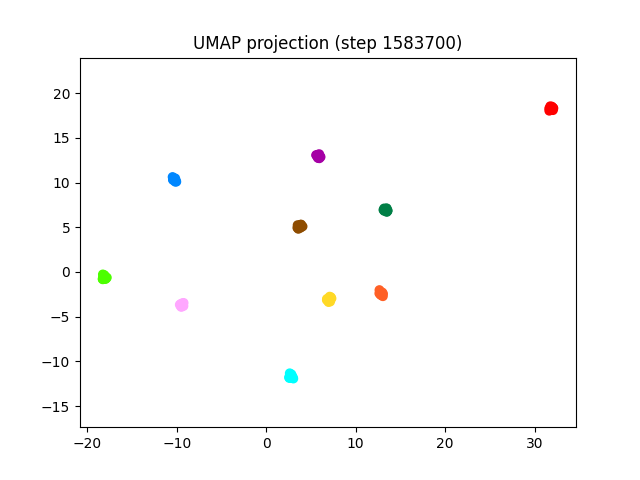
\includegraphics[width=1\linewidth]{\picPath/encoder_umap_1583700.png}
\end{center}
  \caption{Результат работы модели LSTM на обучающих данных на шаге тренировки 158370, спроецированный на плоскость при помощи метода UMAP\cite{bib:umap}. Точки одного цвета относятся к аудиозаписям одного спикера}
  \label{pic:umap_lstm}
\end{figure}


Этап тренировки модели генерации MEL спектрограмм, кроме непосредственно текста для генерации, требует на вход выход модели идентификации спикера. Поэтому перед началом этого этапа для каждой аудиозаписи генерируется соответствующий ему выходной вектор натренированной модели с предыдущего этапа. Этот вектор, в последствии, используется как входной признак для модели генерации MEL спектрограмм. График значений функции ошибки изображен на рисунке \ref{pic:training_graph_tacotron}. Пример спектрограммы, полученный в результате генерации, сопоставленный с соответсвующей спектрограммой из обучающего набора данных представлена на рисунке  \ref{pic:spectrogram_generated}. 


Модель генерации звукового сигнала требует на вход MEL спектрограмму, полученную с предыдущего этапа работы модели, поэтому в тренировочный датасет для модели генерации аудио сигнала добавляется еще и выход натренированной модели генерации MEL спектрограмм. График значений функции ошибки во время тренировки изображен на рисунке \ref{pic:training_graph_wavernn}. Как видно из рисунка \ref{pic:spectrogram_generated}, сгенерированная спектрограмма незначительно отличается от оригинальной. Третий этап генерации звуковых сигналов не только решает задачу оценки фазовых значений для блоков спектрограммы, но и работает как фильтр для исправления незначительных дефектов модели генерации.  

\begin{figure}[H]
\begin{center}
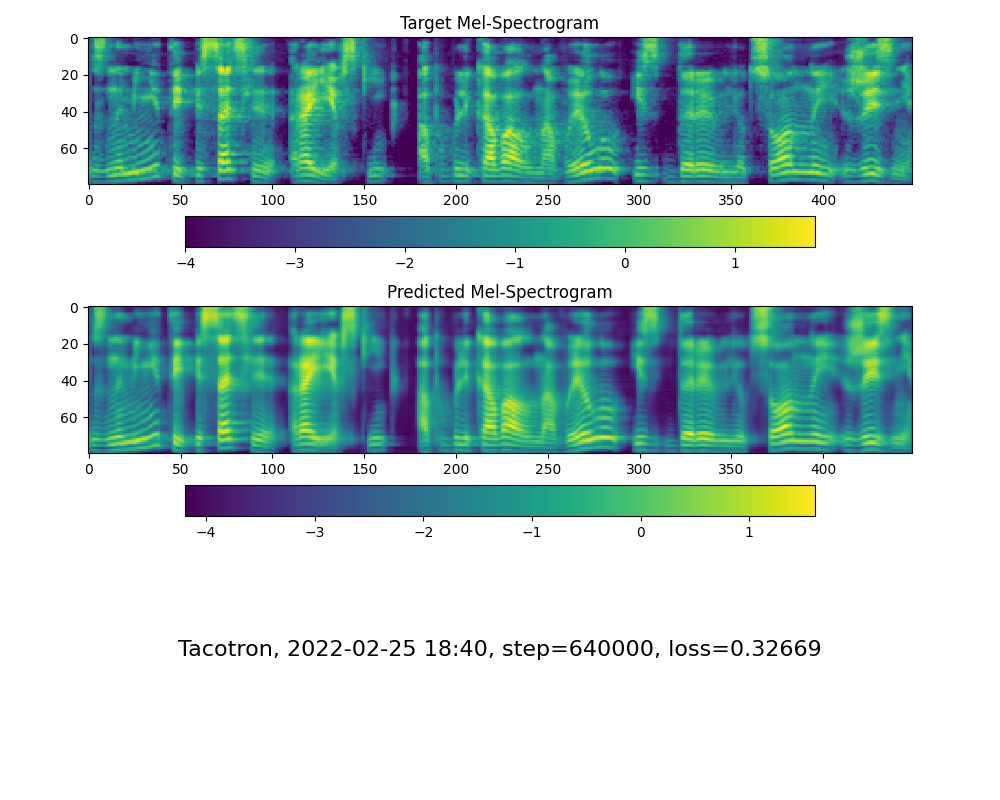
\includegraphics[width=0.85\linewidth]{\picPath/step-640000-mel-spectrogram_sample_1.png}
\end{center}
  \caption{Сравнение сгенерированной MEL спектрограммы с соответсвующей спектрограммой из тренировочного датасета на 640000 шаге тренировки модели Tacotron 2}
  \label{pic:spectrogram_generated}
\end{figure}



\begin{figure}[H]
  \centering
  \begin{subfigure}[b]{1.0\linewidth}
    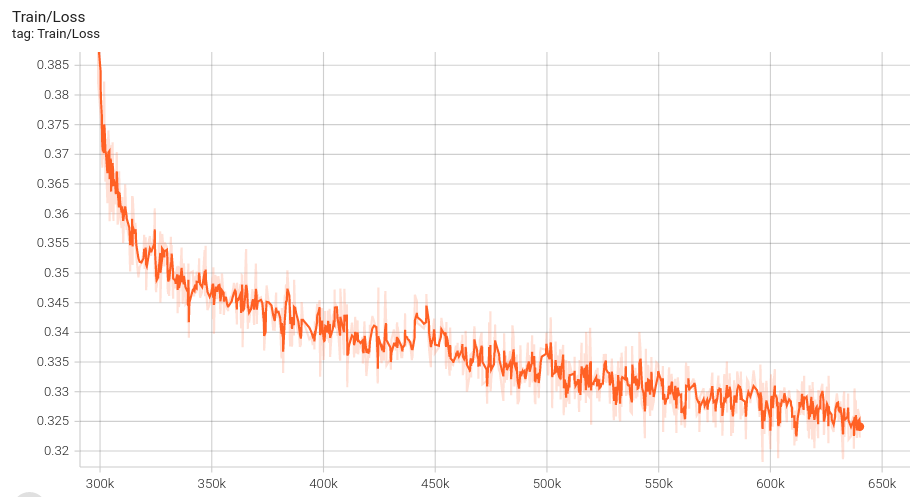
\includegraphics[width=\linewidth]{\picPath/tacotron_tensorboard_steps.png}
    \caption{График значений функции ошибки Tacotron 2 во время тренировки}
    \label{pic:training_graph_tacotron}
  \end{subfigure}
   \begin{subfigure}[b]{1.0\linewidth}
    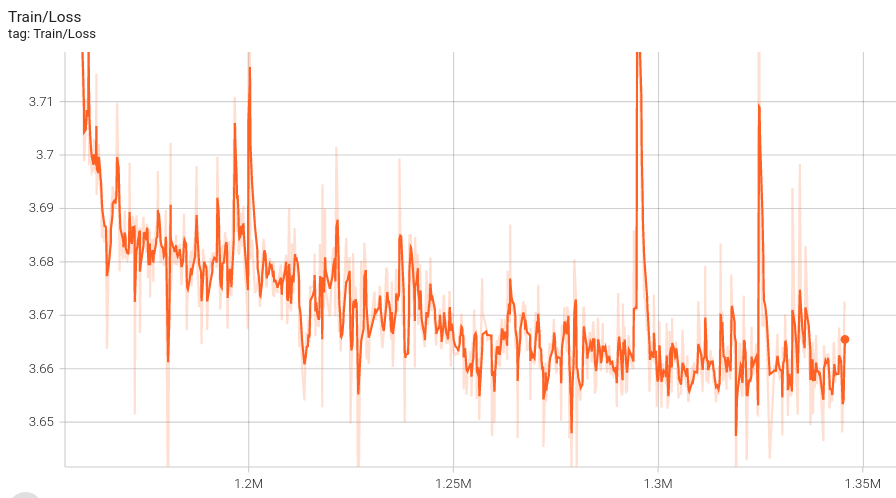
\includegraphics[width=\linewidth]{\picPath/waweRNN_tensorboard_steps.png}
    \caption{График значений функции ошибки WaveRNN во время тренировки}
 \label{pic:training_graph_wavernn}
  \end{subfigure}
  \caption{Графики функций ошибки для моделей Tacotron 2 генерации MEL спектрограмм и WaveRNN генерации аудиофайлов с экспоненциальным усреднением с коэффициентом 0.6}
  \label{pic:training_graphs}
\end{figure}


Несмотря на ограниченность данных модель оказалась способна генерировать внятную речь в том случае, когда голос спикера на входящей аудиозаписи субъективно несколько совпадает с голосом некоторого спикера из тренировочной выборки. Однако в случае, когда субъективно похожего голоса из тренировочных данный не находится - модель не справляется с качественной генерацией длинных текстов, добавляя в вывод различные артефакты. Для улучшения качества генерации на данном этапе была предложена эвристика, описанная в главе \ref{chap:heuristic}. Главный вывод тренировки - для некоторого множества спикеров модель, несмотря на небольшой объем тренировочных данных, способна генерировать внятную речь.


\iffalse
В попытке улучшить качество генерации в качестве модели, решающей задачу идентификацию спикера, вместо имеющегося LSTM была использована Resnet подобная архитектура. Чекпуинта не нашлось, к сожалению, для resnet, поэтому затею бросил
\fi
\section{Эвристика для улучшения генерации голоса в условиях ограниченности датасета}
\label{chap:heuristic}
Тренировочный датасет ограничен, и, как показывате практика, голоса с определенными особенностями (например, высокий женский голос) могут быть не представлены в тренировочной выборке. В результате, пытаясь повторить редкий в тренировочном датасете голос, модель может генерировать некачественный вывод, в котором сложно разобрать слова или присутствует множество артефактов. Однако при клонировании голосов, близких по характеристикам к голосам спикеров из тренировочного датасета, подобные артефакты встречаются редко.  Для уменьшения подобных дефектов генерации автором этой работы предложен метод, суть которого заключается в линейном смешивании векторов спикеров с векторами из тренировочного датасета. Под векторами спикеров в этой главе понимаются выходы модели идентификации спикера для соответствующих входов - аудиозаписей спикеров.  

Алгоритм устроен следующим образом: в наборе латентных векторов спикеров из тренировочного датасета находится вектор, максимально близкий по косиноснуму расстоянию к данному вектору. Затем найденный вектор смешивается в некоторой пропорции, в зависимости от желания сохранить больше особенностей речи или сделать её более четкой и понятной, с вектором спикера. Таким образом, если во время тренировки модель "не слышала" голос, похожий на голос спикера, можно сделать генерацию более похожей на ту, которая присутствует в тренировочном датасете. Формально процедура выше описывается формулой  \ref{eq:vec_mix}:

$$
\begin{equation}
\mathbf{x_{mix}}(\mathbf{x}) = m \cdot \mathbf{x} + (1-m) \cdot \mathbf{x_{c(\mathbf{x})}}
\label{eq:vec_mix}
\end{equation}
$$

где $\mathbf{c}$ определяется из формулы \ref{eq:closest}:

$$
\begin{equation}
\mathbf{c}(\mathbf{x}) = \arg \min_i \frac{|  \mathbf{x} \cdot \mathbf{x_i}|}{\|\mathbf{x}\|\|\mathbf{x_i}\|}
\label{eq:closest}
\end{equation}
$$

где $m \in [0, 1]$ и набор$\{\mathbf{x_i}\}$ - центроиды векторов спикеров из тренировочного датасета,  полученых в результате работы модели идентификации спикера. Центроиды могут быть предвычислены заранее, и дополнительное замешивание  не потребует большого количества операций во время инференса модели. Параметр $m$ можно подбирать в ручную, однако можно также определить его как зависимым от модуля косинусного расстояния между $\mathbf{x}$ и $\mathbf{x_c}$, например так, как в формуле \ref{eq:sigma}:

$$
\begin{equation}
m 
= 
m(\mathbf{x})
=
2 \sigma (k \cdot
\mathbf{x_{c(x)}})
- 1
\label{eq:sigma}
\end{equation}
$$

где чем больше коэффициент $k$ - тем сильнее вектор из тренировочного набора будет преобладать над вектором, полученным из входных данных.


Благодаря этой эвристике можно несколько улучшить качество генерации в ущерб уникальным характеристикам входного голоса. В случае, когда вектор входного голоса находится достаточно далеко от всех центроидов тренировочных векторов и сгенерированная речь субъективно неразборчива, применение эвристики помогает получить субъективно лучший результат. 


Другой способ улучшить качество генерации - использовать несколько аудиозаписей для генерации латентных векторов спикеров. Как показывает практика, запуская модель идентификации на нескольких разных аудиозаписях одного спикера и усредняя результат, можно получить вектор, содержащий больше полезных характеристик голоса спикера, и, как результат, качество генерации голоса станет субъективно лучше.

\section{Пользовательский интерфейс}
Для удобной работы с моделью клонирования голоса может быть использован графический интерфейс, изображенный на рисунке \ref{pic:gui}, или консольное приложение. 
\iffalse Кроме того, с развернутой в облаке моделью можно взаимодействовать через телеграм бота, описаного ниже. 
\fi
\begin{figure}[H]
\begin{center}
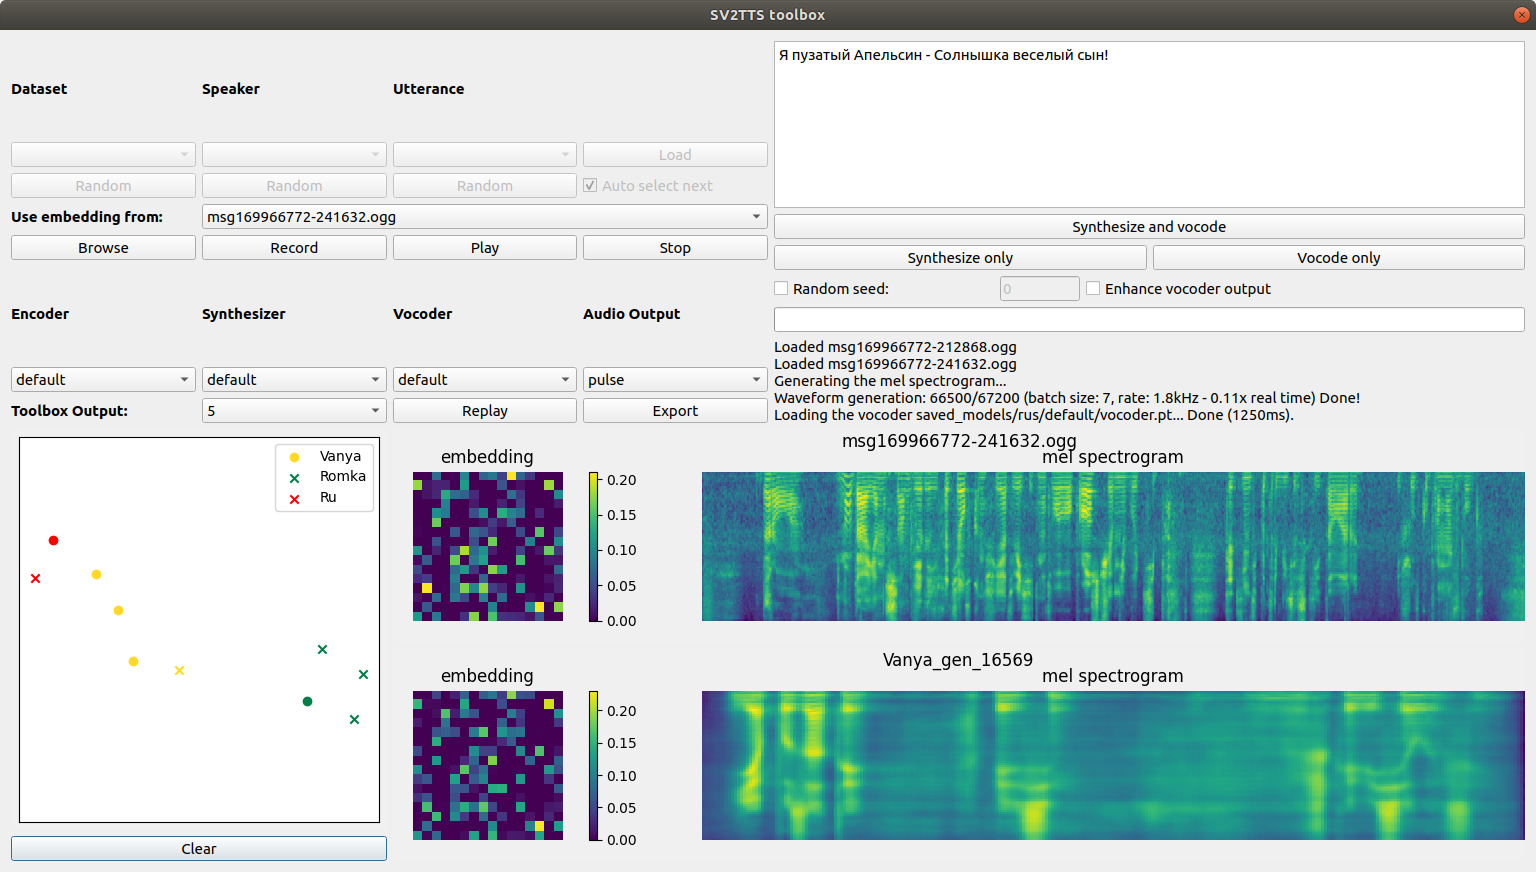
\includegraphics[width=1.\linewidth]{\picPath/gui.png}
\end{center}
  \caption{Пользовательский интерфейс модели клонирования голоса}
  \label{pic:gui}
\end{figure}

Для запуска графического интерфейса необходимо установить зависимости и указать пути до тренировочного датасета и сохраненных весов моделей. Подробную инструкцию по запуску можно найти в описании рабочего репозитория.

Графический интерфейс имеет следующие составляющие: левая верхняя часть  отвечает за загрузку аудиозаписей, голос из которых затем можно склонировать, и загрузку весов моделей. В верхнем блоке располагаются кнопки для загрузки данных из датасетов, в нижней - кнопки для загрузки произвольных аудиозаписей. Ниже находится блок выбора весов модели и устройства вывода. В качестве последнего этапа генерации аудиофайлов можно использовать алгоритм Гриффина-Лимма, выбрав соответсвующий пункт в меню Vocoder.

Правая верхняя часть интерфейса отвечает за ввод текста для генерации и непосредсвенно за генерацию звука. Кнопка Synthesize запускает модель генерации MEL-спектрограмм, а кнопка Vocode only генерирует звуковой сигнал из текущей MEL-спектрограммы. Кнопка synthesize and vocode позволяет получить сразу и MEL-спектрограмму, и аудиофайл.

Нижняя часть интерфейса отвечает за визуализацию: в левом нижнем углу располагается визуализация UMAP проекции\cite{bib:umap} латентных векторов загруженных аудиофайлов, полученных при помощи модели идентификации спикера. Разными цветами обозначены разные спикеры, круг означает, что вектор получен из оригинальной дорожки, а крест означает, что вектор получен из сгенерированной аудиодорожки. Правее находятся визуализации спектрограмм и их векторного представления. Верхняя пара изображений относится к входному аудиофайлу, а нижняя -  к сгенерированному в текущий момент аудиофайлу. 

Для клонирования голоса необходимо сначала загрузить входной аудиофайл при помощи кнопки Browse или записать его с доступного устройства ввода при помощи кнопки Record. Преред генерацией запись можно прослушать, используя для управления кнопки Play и Stop. После загрузки аудиофайла программа автоматически преобразовывает его в MEL сперктрограмму, генерирует латентный вектор, используя модель идентификации спикеров, и визуализирует спектрограмму, латентный вектор и его UMAP проекцию в нижней части интерфейса. После этого необходимо ввести требуемый для генерации текст в окно ввода текста в верхнем правом углу. Используя интерфейс для генерации и выбирая нужные веса для модели, можно получить сгенерированный аудиофайл, для генерации которого использовался введенный ранее текст и латентный вектор загруженного ранее целевого аудиофайла. Визуализации сгенерированного файла автоматически отобразится в нижней части программы. Результат генерации можно прослушать заново, используя кнопку Replay или сохранить на диск, используюя кнопку Export. 

Для генерации нескольких аудиозаписей с разным текстом для множества спикеров удобно использовать консольную программу demo_advanced.py. Программа позволяет использовать текстовый файл в качестве входа, интерпретируя каждую строчку как отдельный текст для генерации. Входные аудиозаписи должны соответствовать следующей структуре папок: аудиозаписи каждого спикера хранятся в отдельной директории, название директории соответствует имени спикера. Как было описано в главе \ref{chap:heuristic}, генерация, использующая усредненные латентные вектора разных аудиозаписей, работает субъективно лучше, и в консольной программе существует возможность агрегации латентных векторов: для этого необходимо загрузить несколько аудиофайлов в папку спикера и передать в программу параметр, соответствующий режиму агрегации латентных векторов. Кроме того, программу можно запустить в режиме смешения, когда вектора спикеров линейно смешиваются с векторами из тренировочного датасета. Подробное описание алгоритма можно найти в главе \ref{chap:heuristic}. Подробное описание всех режимов работы можно найти в описании рабочего репозитория.

\section{Валидация модели клонирования голоса}
\label{chap:results}
Для проверки качества работы модели клонирования голоса использовались 10 текстов и 14 спикеров, не входивших в тренировочный набор данных. В качестве метрики оценки качества используется cредняя оценка экспертов (Mean Opinion Score) по двум характеристикам: натуральность речи и схожесть сгенерированного голоса с  оригинальным. Значения оценок - $1, 2, 3, 4, 5$, где $1$ значит низкую оценку характеристики элемента, $5$ - высокую оценку характеристики элемента. Для сбора выбранной метрики автором работы было реализовано веб приложение, код которого находится в директории questionnaire основного репозитория работы. 

Результаты сравнения можно наблюдать в таблице \ref{table:evaluation}. В сравнении используются генерации из репозитория \cite{bib:russian_voice_cloning}и генерации этой работы, представленные в двух режимах: генерация без замешивания, но с усреднением латентных векторов, обозначается в таблице как режим 1,  и генерация с замешиванием и усреднением латентных векторов, обозначается в таблице стравнения как режим 2. 

\begin{table}[H] 
\begin{tabularx}{\textwidth}{|X|X|X|}
\hline
Режим генерации
&
Средняя оценка качества генерации
&
Средняя оценка схожести голосов
\\
\hline
Multi Tacotron Voice Cloning \cite{bib:russian_voice_cloning}
&
1.93
 &
 1.3
\\
\hline
Модель этой работы в режиме 1
&
3.28
&
{\bf 2.69}
\\
\hline
Модель этой работы в режиме 2
&
{\bf 3.74}
 &
2.49
\\
\hline
\end{tabularx}
\caption{Результат сравнения генераций предшествующей  модели и модели этой работы в двух разных режимах генерации}
\label{table:evaluation}
\end{table}

Как видно из таблицы \ref{table:evaluation}, в обоих режимах генерации модель, полученная автором этой работы, превосходит предыдущую версию модели как по качеству генерации, так и по оценки схожести оригинальных и сгенерированных голосов.  Кроме того из таблицы можно видеть, что эвристика, представленная в главе \ref{chap:heuristic}, как и предполагалось, улучшает оценку качества генерации уменьшая при этом оценку схожести сгенерированных голосов. 

\chapter{Вывод}
В результате работы были изучены методы хранения, обработки и преобразования аудиофайлов в цифровом виде. Исследована задача клониравния голоса, включающая в себя такие подзадачи, как задача идентификации спикера, задача генерации MEL-спектрограмм и задача генерации аудиосигнала на основе MEL-спектрограмм. Собраны и предобработаны датасеты для тренировки каждой из подзадач, запущена сама тренировка моделей решения задач клонирования голоса.

В качестве основы была использована кодовая база репозитория\cite{bib:voice_cloning}, однако в процессе работы были выявлены ошибки и недоработки, исправленные автором, улучшен интерфейс логирования статистик тренировки, а также переработаны все фрагменты кода препроцессинга данных, так как предыдущая версия не подразумевала работу с несколькими датасетами, имеющими разную структуру хранения данных. Была выполнена тренировка и последующая валидация моделей для клонирования голоса. В условиях малого набора обучающих данных были разработаны и реализованы эвристики, позволяющие улучшить качество генерации модели клонирования голоса. Произведено сравнение качества генерации обученной модели с конкурирующей версией\cite{bib:russian_voice_cloning}, в результате которого натренированная автором этой работы модель получила оценку выше конкурирующей модели. Для использования модели был подготовлен графический и консольный интерфейс модели клонирования голоса, позволяющий пользователям клонировать произвольный голос, визуализировать латентные вектора и MEL-спектрораммы и подбирать коэффициенты для эвристик улучшения генерации. 
\newpage
%список литературы
\addcontentsline{toc}{chapter}{Список использованных источников}
\begin{thebibliography}{0}

\bibitem{bib:voice_cloning} Jia, Ye and Zhang, Yu and Weiss, Ron J. and Wang, Quan and Shen, Jonathan and Ren, Fei and Chen, Zhifeng and Nguyen, Patrick and Pang, Ruoming and Moreno, Ignacio Lopez and Wu, Yonghui: Transfer Learning from Speaker Verification to Multispeaker Text-To-Speech Synthesis. 2018. arXiv 1806.04558

\bibitem{bib:web_audio} Josh Beggsl, Dylan Thede: Designing Web Audio. ISBN 1-56592-353-7 $-$ М: O`REILLY, 2001. Источник $-$ docstore.mik.ua/orelly/web2/audio/index.html

\bibitem {Gonzalez}
  Gonzalez R.C.,  Woods R.E. Processing digital Image 4 global edition $-$ M: Pearson, 2017. $-$ 993с.

\bibitem{bib:bio_signals_and_image_proc} 
Kay van Najarian, Robert Splinter: Biomedical SignalandImage Processing. 2012. Taylor \& Francis Group, DOI 10.1201/b11978. $-$ 441 с.


\bibitem{bib:think_DSP} Allen B. Downey: Think DSP $-$ M: Green Tea Press, 2014. $-$ 153 c.

\bibitem{bib:librosa} Brian McFee, Colin Raffel, Dawen Liang, Daniel, Patrick Whittlesey Ellis, Matt McVicar, Eric Battenberg, Oriol Nieto: Librosa: Audio and music signal analysis in Python  14th PYTHON IN SCIENCE CONF. (SCIPY 2015) $-$ 2015.

\bibitem{bib:MFCC} S. B. Davis and P. Mermelstein: Comparison of parametric representations for monosyllabic word recognition in continuously spoken sentence, IEEE, Trans. Acoust. Speech Signal Processing, том 28, \textnumero 4, с. 357–366, 1980.

\bibitem{bib:MFCC_choice}M., Laxmi Narayana and Kopparapu, Sunil Kumar: Choice of Mel Filter Bank in Computing MFCC of a Resampled Speech. 2014. arXiv 1410.6903

\bibitem{bib:lstm} Sepp Hochreiter and Jurgen Schmidhuber: Long short-term memory. Neural computation, том. 9, \textnumero 8, с. 1735–1780, 1997.

\bibitem{bib:e2e_speaker_ver_loss} Wan, Li and Wang, Quan and Papir, Alan and Moreno, Ignacio Lopez: Generalized End-to-End Loss for Speaker Verification. 2017. arXiv 1710.10467

\bibitem{bib:Tacotron} Yuxuan Wang, RJ Skerry-Ryan, Daisy Stanton, Yonghui Wu, Ron J. Weiss, Navdeep Jaitly, Zongheng Yang, Ying Xiao, Zhifeng Chen, Samy Bengio, Quoc Le, Yannis Agiomyrgiannakis, Rob Clark, Rif A. Saurous: Tacotron: Towards End-to-End Speech Synthesis. 2017. arXiv 1703.10135

\bibitem{bib:pytorch} Paszke, Adam and Gross, Sam and Massa, Francisco and Lerer, Adam and Bradbury, James and Chanan, Gregory and Killeen, Trevor and Lin, Zeming and Gimelshein, Natalia and Antiga, Luca and Desmaison, Alban and Köpf, Andreas and Yang, Edward and DeVito, Zach and Raison, Martin and Tejani, Alykhan and Chilamkurthy, Sasank and Steiner, Benoit and Fang, Lu and Bai, Junjie and Chintala, Soumith: PyTorch: An Imperative Style, High-Performance Deep Learning Library. 2019. arXiv 1912.01703

\bibitem{bib:resnet} He, Kaiming and Zhang, Xiangyu and Ren, Shaoqing and Sun, Jian: Deep Residual Learning for Image Recognition. 2015. arXiv 1512.03385
\bibitem{bib:highway_net} Rupesh Kumar Srivastava, Klaus Greff, Jürgen Schmidhuber: Highway Networks. 2015. arXiv 1505.00387

\bibitem{bib:GRU} Junyoung Chung, Caglar Gulcehre, KyungHyun Cho, and Yoshua Bengio. Empirical evaluation of gated recurrent neural networks on equence modeling. 2014. arXiv:1412.3555

\bibitem{bib:attention} Oriol Vinyals, Łukasz Kaiser, Terry Koo, Slav Petrov, Ilya Sutskever, and Geoffrey Hinton: Grammar as a foreign language. In Advances in Neural Information Processing Systems, с. 2773–
2781, 2015.

\bibitem{bib:LSTM} Staudemeyer, Ralf C. and Morris, Eric Rothstein: Understanding LSTM -- a tutorial into Long Short-Term Memory Recurrent Neural Networks. 2019. arXiv 1909.09586

\bibitem{bib:teacher_forcing} John F. Kolen; Stefan C. Kremer :A Field Guide to Dynamical Recurrent Networks. John Wiley & Sons. с. 202–. ISBN 978-0-7803-5369-5. 2001

\bibitem{bib:phase_estim} D. Griffin, J. Lim: Signal estimation from modified shorttime Fourier transform. IEEE Trans. Acoust., Speech, Signal Process., Том 32, \textnumero 2, с. 236–243. 1984.

\bibitem{bib:wavenet} Oord, Aaron van den and Dieleman, Sander and Zen, Heiga and Simonyan, Karen and Vinyals, Oriol and Graves, Alex and Kalchbrenner, Nal and Senior, Andrew and Kavukcuoglu, Koray: WaveNet: A Generative Model for Raw Audio. 2016. arXiv 1609.03499

\bibitem{bib:waveRNN} Kalchbrenner, Nal and Elsen, Erich and Simonyan, Karen and Noury, Seb and Casagrande, Norman and Lockhart, Edward and Stimberg, Florian and Oord, Aaron van den and Dieleman, Sander, Kavukcuoglu, Koray: Efficient Neural Audio Synthesis. 2018. arXiv 1802.08435

\bibitem{bib:Ruslan} Gabdrakhmanov L., Garaev R., Razinkov E. (2019) RUSLAN: Russian Spoken Language Corpus for Speech Synthesis. In: Salah A., Karpov A., Potapova R. (eds) Speech and Computer. SPECOM 2019. Lecture Notes in Computer Science, vol 11658. Springer, Cham


\bibitem{bib:open_tts} Russian Open Speech To Text (STT/ASR) Dataset : сайт репозитория. $-$  URL: https://github.com/snakers4/open_stt (дата обращения: 10.05.2022 ). 

\bibitem{bib:librispeech} LibriSpeech ASR corpus: официальный сайт. $-$ URL: http://www.openslr.org/12/ (дата обращения: 10.05.2022).

\bibitem{bib:vox_celeb} A. Nagrani, J. S. Chung, W. Xie, A. Zisserman: Voxceleb: Large-scale speaker verification in the wild. 2019. $-$ URL: https://www.sciencedirect.com/science/article/pii/S0885230819302712. Computer Science and Language.

\bibitem{bib:Mozilla} Mozilla Common Voice Dataset: оффициальный сайт. $-$ URL: https://commonvoice.mozilla.org/en/datasets (дата обращения: 10.05.2022).

\bibitem{bib:russian_single} Russian Single Speaker Speech Dataset: страница датасета. $-$ URL: https://www.kaggle.com/datasets/bryanpark/russian-single-speaker-speech-dataset (дата обращения: 10.05.2022).

\bibitem{bib:umap} McInnes, Leland and Healy, John and Melville, James: UMAP: Uniform Manifold Approximation and Projection for Dimension Reduction. 2018. arXiv 1802.03426

\bibitem{bib:Danya_voice_cloning} Tacotron Voice Cloning Rus: сайт репозитория.  URL - https://github.com/dupeljan/Real-Time-Voice-Cloning

\bibitem{bib:russian_voice_cloning} Multi-Tacotron Voice Cloning (Russian/English): сайт репозитория. URL $-$ https://github.com/vlomme/Multi-Tacotron-Voice-Cloning (дата обращения: 10.05.2022).

\end{thebibliography}

\end{document}